\documentclass[a4paper,openright,twoside,11pt]{report}

% % Include packages % %

% Basic
\usepackage[english]{babel}		% Document language
\usepackage[utf8x]{inputenc}	% Character encoding
\usepackage{appendix}			% Increases control of appendices

% Standard colors
\PassOptionsToPackage{dvipsnames}{xcolor}
	\RequirePackage{xcolor} % [dvipsnames]

% Figures
\usepackage{float}				% Improves handling of floating objects
\usepackage[pdftex]{graphicx}	% Improves handling of graphics
\usepackage{pdfpages}			% Allows inclusion of entire PDF
\usepackage{tikz}				% Allows construction of diagrams

% Tables
\usepackage{multicol}			% Allows multi-columns in tables
\usepackage{multirow}			% Allows multi-rows in tables

% Math
\usepackage{amsmath}			% Adds functionality to math environments
\usepackage{amssymb} 			% Adds to more symbols to math environments

% Listings
\usepackage{listings}			% Allows the use of listings

% Misc
\usepackage{xspace}				% Allows spaces after commands
\usepackage{todonotes}			% Enable todo notes
\usepackage{booktabs}			% Various optimizations to LaTeX
\usepackage{lastpage}			% Allows reference to LastPage 
\usepackage{type1cm}			% Increase flexibility of font sizes
\usepackage{enumerate}			% Allows one to choose the style of an enumeration
\usepackage[square,numbers]{natbib}
\bibliographystyle{unsrt}

% Hyperlinks
\usepackage[hyphens]{url}		% Create URL's with line breaks
\usepackage{hyperref}			% Allows hyperlinks
\usepackage{bookmark}

% Clever refs - although not clever enough to be included before hyperref....
\usepackage{cleveref}     % Adds intelligent references ("Figure F1-2", instead of "F1-2")

% ADD THESE LAST BECAUSE OF PACKAGE DEPENDENCIES!
%[LABEL] pagelayout
%[DESCRIPTION] Defines the page headers and whitespace placement.

%[BEGIN] Define page headers and footers
  %[BEGIN] Load fancy headers package
    \usepackage{fancyhdr}
  %[END]
  
  % Document visual header definition
	\setlength{\headheight}{15pt}
 	
 	\pagestyle{fancy}
	\renewcommand{\chaptermark}[1]{\markboth{\small{\scshape{#1}}\ \scshape{\small{\thechapter}}}{}}
	\renewcommand{\sectionmark}[1]{\markright{\scshape{\small{\thesection}}\ \small{\scshape{#1}}}}

	\fancyhf{}
	\fancyhead[LE,RO]{\thepage}
	\fancyhead[LO]{\rightmark}
	\fancyhead[RE]{\leftmark}
	
	\renewcommand{\headrule}{{\color{black}%
  \hrule width\headwidth height\headrulewidth \vskip-\headrulewidth}}
	\renewcommand{\headrulewidth}{0.3pt}
	\renewcommand{\footrulewidth}{0pt}

	\addtolength{\headheight}{0.5pt}
	\setlength{\footskip}{0in}
	\renewcommand{\footruleskip}{0pt}
	\fancypagestyle{plain}{%
		\fancyhead{}
		\renewcommand{\headrulewidth}{0pt}
	}
%[END]

%[BEGIN] Chapter customisation
  \usepackage{graphics}
  \usepackage{titlesec}
  \titleformat{\chapter}[display]
    {\normalfont\Large\raggedleft}
    {\MakeUppercase{\chaptertitlename}%
      \rlap{\resizebox{!}{1.5cm}{~\thechapter~} \rule{5cm}{1.5cm}}}
    {10pt}{\Huge\bf}
  \titlespacing*{\chapter}{0pt}{30pt}{20pt}
%[END]

%[BEGIN] Bibliography in TOC
  \usepackage[nottoc]{tocbibind} % Works only with standard classes
%[END]

%[BEGIN] Margin adjustment
  \usepackage[total={5in,8.75in},top=1in,left=1.5in,bottom=1.0in]{geometry}
%[END]

%[BEGIN] define whitespace placement
  \raggedbottom
%[END]

% Numbering
\renewcommand{\thesection}{\arabic{chapter}.\arabic{section}}
\renewcommand{\thesubsection}{\thesection.\arabic{subsection}}
\renewcommand{\thesubsubsection}{\thesubsection.\arabic{subsubsection}}
\renewcommand{\thefigure}{F\arabic{chapter}-\arabic{figure}}
\renewcommand{\thetable}{T\arabic{chapter}-\arabic{table}}

% Counters
\setcounter{tocdepth}{1}
\setcounter{secnumdepth}{3}
		% Layout definitions
% Part descriptions
% Usage \newpart{part name}{part text}
\newcommand{\newpart}[2]{
	\part[#1]{#1\\
		\begin{minipage}[c]{10cm}
		\centering
		\vspace{2cm}
		\normalsize{\textnormal{
			\textit{#2}
		}}
		\end{minipage}
	}
}

% Insert figure
\newcommand{\insertfigure}[4]{%
    \begin{figure}[H] %
        \center %
        \includegraphics[#1]{figures/#2} %
        \caption{#3} %
        \label{#4} %
        \vspace{-5pt}
    \end{figure} %
}

% Insert figure
\newcommand{\inserttexfigure}[3]{%
    \begin{figure}[H] %
        \center %
        \input{figures/#1} %
        \caption{#2} %
        \label{#3} %
        \vspace{-5pt}
    \end{figure} %
}

% Allow line break in texttt
\newcommand*\justify{%
  \fontdimen2\font=0.4em% interword space
  \fontdimen3\font=0.2em% interword stretch
  \fontdimen4\font=0.1em% interword shrink
  \fontdimen7\font=0.1em% extra space
  \hyphenchar\font=`\-% allowing hyphenation
}

\let\oldtexttt\texttt
\renewcommand*{\texttt}[1]{\oldtexttt{\justify #1}}

% Add Blankpage command
\newcommand{\Blankpage}{ %
    \newpage               %
    \thispagestyle{empty}  %
    \mbox{}                %
    \newpage               %
}

% TODO NOTES COMMANDS
\newcommand{\namedtodo}[5]
{
  \stepcounter{todocounter}
  \ifthenelse{\equal{#1}{inline}}
  % INLINE TODO
  {
    \todo[color=#4,caption={\textbf{\inserttodocounter #3: } #2},inline]
    {\textbf{\inserttodocounter #3: }\color{#5}#2}
  }
  % NORMAL TODO
  {
    \todo[color=#4,caption={\textbf{\inserttodocounter #3: } #2}]
    {\textbf{\inserttodocounter #3: }\color{#5}#2}
  }
}
% Counter format
\newcommand{\inserttodocounter}{\#\thetodocounter\;}

% FORMAT FOR TODO:
% [inline] (optional) besked navn bg-farve font-farve
\newcommand{\vagner}[2][]{\namedtodo{#1}{#2}{Vagner}{CarnationPink}{black}}
\newcommand{\thilemann}[2][]{\namedtodo{#1}{#2}{Stefan T}{NavyBlue!35}{black}}
\newcommand{\jesper}[2][]{\namedtodo{#1}{#2}{Jesper}{green}{black}}
\newcommand{\frederik}[2][]{\namedtodo{#1}{#2}{Frederik}{red!90}{black}}

%GIRAF commands
\newcommand{\giraf}{GIRAF\xspace}
\newcommand{\launcher}{Launcher\xspace}		% Custom commands and environments
% FIGURES
\graphicspath{{figures/}{../figures/}}

% Define hyperef style
\hypersetup %
{
	colorlinks=true,
	linktocpage=true, 
	pdfstartpage=1,
	pdfstartview=FitV,
	hypertexnames=true,
	pdfhighlight=/O,
	breaklinks=true,
	pdfpagemode=UseNone,
	pageanchor=true,
	pdfpagemode=UseOutlines,
	plainpages=false,
	bookmarksnumbered,
	bookmarksopen=true,
	bookmarksopenlevel=1,
	bookmarksdepth=2,
	urlcolor=NavyBlue,
	linkcolor=Red,
	citecolor=Red,
	pdfborder={0 0 0},
}

\lstset %
{
	language=Java,
	keywordstyle=\color{RoyalBlue},
    commentstyle=\color{Green}\ttfamily,
    stringstyle=\color{Red}\ttfamily,
	frame=shadowbox,
	framesep=5pt,
	aboveskip=1.5em,
	belowskip=1em,
	rulecolor=\color{blue!40!black},
	rulesepcolor=\color{white!93!black},
	basicstyle=\ttfamily\normalsize,
	numbers=left,
	numberstyle=\tiny,
	numberfirstline=true,
	numberblanklines=false,
%	showstringspaces=false,
	stepnumber=1,
	numbersep=9pt,	
	captionpos=b,
	escapeinside={(*}{*)},
	breaklines=true,
	breakatwhitespace=true,
	alsoletter={;}
}

% TIKZ
\usetikzlibrary{positioning,fit,calc,shapes,arrows,external,petri}
\tikzset{
    state/.style={
		rectangle,
		rounded corners,
		draw=black, very thick,
		minimum height=2em,
		inner sep=2pt,
		text centered
	},
    layer/.style={
		rectangle,
		rounded corners,
		draw=black, very thick,
		minimum height=4em,
    	minimum width=10cm,
		inner sep=2pt,
		text centered
   },
    dummy/.style={
		rectangle,
		rounded corners,
		minimum height=2em,
		inner sep=2pt,
		text centered
   },
	lbl/.style={
		above,
		sloped % make the text follow the path
	}

}

% Make quotes italic
\AtBeginEnvironment{quote}{\itshape}			% Package setup

% Only compile part of the report
% Useful if we want feedback on certain parts/chapters
%\includeonly{documents/01-Front/index,documents/03-Sprint1/index}

\begin{document}

% Remember to disable todonotes entirely in final version
% It can be done explicitly in preamble by passing 
% options [disable] to the todonotes package
\newcounter{todocounter}
\listoftodos

% Introduction
\pagenumbering{roman}
\pagestyle{empty}
%% Use this for frontpage image
%\includepdf[noautoscale]{figures/frontpage.pdf}
\phantomsection
\thispagestyle{empty}

\newcommand{\HRule}{\rule{\linewidth}{0.5mm}} % Defines a new command for the horizontal lines, change thickness here

\begin{center}
\textsc{}\\[0.5cm]

\textsc{\LARGE Aalborg Universitet}\\[0.8cm]
\textsc{\Large SW6 Project}\\[0.4cm]
\textsc{\large Developing Complex Software Systems}\\[0.4cm]

\HRule \\[0.4cm]
{ \huge \bfseries Software for Children with Autism}\\[0cm]
\HRule \\[0.8cm]
\begin{minipage}{0.4\textwidth}
\begin{flushleft} \large
\emph{Group:}\\
Jesper Byrdal Kjær\\
Frederik Bruhn Mikkelsen\\
Stefan Mailund Thilemann\\
Anders Vagner
\end{flushleft}
\end{minipage} 
~
\begin{minipage}{0.4\textwidth}
\begin{flushright} \large
\emph{Supervisor:}\\
Hua Lu
\end{flushright}
\end{minipage}\\[1.5cm]

%\includegraphics[width=\textwidth]{figures/legoCar.jpg}\\[1cm]

%{\large 20-12-2013}\\[0cm]

\vfill

\includegraphics[height=3cm]{figures/aauLogoEnStudent.png}
\vfill

\end{center}


\Blankpage
\phantomsection
\thispagestyle{empty}
\label{chap:titelpage}
\pdfbookmark{Titlepage}{chap:titlepage}

% Titlepage [START]
    \sectionmark{Titlepage}

    \begin{tabular}{r}
        \parbox{\textwidth}{\raisebox{-15mm}{
\includegraphics[height=3cm]{figures/aauLogoEnStudent.png}} %
         \hfill \parbox{4.9cm}{ %
            \begin{tabular}{l} 
                {\textsf{\small{\textbf{Department of Computer Science}}}}\\
                {\textsf{\small{\textbf{Software 5th semester}}}}\\
                {\textsf{\small{Address: Selma Lagerlöfs Vej 300}}} \\
                {\textsf{\small{\hspace{13 mm} 9220 Aalborg Øst }}} \\
                {\textsf{\small{Phone no.: 99 40 99 40}}} \\
                {\textsf{\small{Fax no.: 99 40 97 98}}} \\
                {\textsf{\small{Homepage: \url{http://www.cs.aau.dk}}}}
            \end{tabular}}}
    \end{tabular}
    
    \begin{tabular}{cc}
	
        \parbox[3cm]{7cm}{ %
	\vspace{7mm}
            \begin{description}
                \item {\textbf{Project title}:} \\
                    Software for Helping \\
                    Children with Autism \thilemann[inline]{Not consistent!}
                    \hspace{4cm}
                \item {\textbf{Subject}:} \\
                  Developing Complex \\
                  Software Systems
            \end{description}
	\vspace{-4mm}
            \parbox{8cm}{ %
                \begin{description}
                    \item {\textbf{Project periode}:} \\
                        Spring 2014
                    \hspace{4cm}
                    \item {\textbf{Group name}:} \\
                        SW605F14
                    \hspace{4cm}
                    \item {\textbf{Supervisor}:} \\
                        Hua Lu
                    \item {\textbf{Group members}:}\\%\newcommand{\sh}{18pt}\\%
                    Jesper Byrdal Kjær\\[0.20cm]
                    Frederik Bruhn Mikkelsen\\[0.20cm]
					Stefan Mailund Thilemann\\[0.20cm]
					Anders Vagner
                \end{description}
            }
	    \vspace{-4mm}
            \begin{description}
                \item {\textbf{Copies}:} XX
                \item {\textbf{Pages}:} \pageref{LastPage}
                \item {\textbf{Appendices}: XX} 
                \item {\textbf{Finished}: XX} 
            \end{description}
            \vfill 
        } &
        \parbox{7cm}{ %
            %\vspace{.15cm} %
            \hfill %
            \begin{tabular}{l}%
                {\textbf{Abstract}:}\bigskip \\%
                \fbox{ %
                    \parbox{6.2cm}{\bigskip %
                    {\vfill{\small %
                     In cooperation between a number of institutions in Aalborg Municipality, and Aalborg University, an Android system for autistic citizens and their guardians has been in development since 2011.
In January 2014, the project was taken over by the new 6th semester software engineering students, whom this group was a part of.

This report documents the progress of the group SW605F14 collaborating with the 15 other groups working on the project.
As the group mainly picked up the task of the improving \launcher, the main application from which all other applications should be accessed, the report describes the continued analysis, customer collaboration and development on this application.
Furthermore, the challenge of working within a multi-project setting is described, as are the advantages and problems this setting brings.

The project was developed over four sprints, and thus this report is divided into chapters concerning the activities carried out during each sprint.
                        \bigskip}}%
                    }}%
            \end{tabular}%
        }
    \end{tabular}

\vfill
    \noindent{\emph{The material in this report is freely and publicly available, publication with source reference is only allowed with the authors' permission.}}
% Titlepage [END]
\newcommand{\headerPreface}{Preface}
\cleardoublepage
\phantomsection
\pdfbookmark{\headerPreface}{chap:preface}
\chapter*{\headerPreface}\label{chap:preface}

\style[inline]{Write method names as \lstinline!fooBar()!}

\style[inline]{Distinguish between activities as concepts and activities as classes.}

\style[inline]{Present tense.}

\style[inline]{Application names in italics: \textit{Pictooplæser}}

\style[inline]{Terminology: children $\rightarrow$ citizens (not in code). User, guardian.}

\style[inline]{Proper captilisation.}

\style[inline]{Correct quote types.}

\thilemann[inline]{Adjust all intros and summaries according to content.}

\jesper[inline]{Describe new specifications, and refer to old ones.}

This report is created by Software Engineering students as a Bachelor project at Aalborg University, spring semester 2014.
To read and understand the report, it is expected that the reader has a background in Computer Science in the light of the technical contents.
The Android APIs are not described directly in this report and thus the reader is encouraged to explore the introduction to Android given by \citet{androidIntroduction}.

Since multiple project groups are collaborating towards developing a complete system, the structure of this report is divided into chapters that logically follows from working in sprints specified by the multi-project guidelines.
Thus there is a chapter for each sprint, which is further subdivided into:

\begin{description}
\item[Sprint Overview] \hfill \\
In this section we describe the overall goals and activities of the sprint.
\item[Analysis and Design] \hfill \\
In this section we describe the analytical processes and design decisions related to the topics 
\item[Developments] \hfill \\
In this section we describe how we solved the tasks of the sprint.
\item[Sprint Review] \hfill \\
In this section we discuss lessons learned during the sprint, including collaboration problems, and erroneous use of development methods.
\end{description}

Following the chapters describing the four sprints, \cref{chap:collaboration} focuses on the work that is done in collaboration with other groups.
Lastly, the results of the project is presented in \cref{chap:evaluation}.

It is important to note, that the applications in the multi project were renamed during this semester.
As a result, many applications have been given Danish names and will not be translated in this report.

References and citations are given with number notation, for example as: \citet{launcher2011}, or without listing the authors as: \cite{launcher2011}. 

We would like to thank our lecturers and our supervisor, Hua Lu for excellent cooperation during the project work.
\jesper[inline]{Fix this up in the end.}



% Some setup
%\setcounter{page}{4}
\setcounter{secnumdepth}{2}

\cleardoublepage
\phantomsection

%Table of content
\pdfbookmark{\contentsname}{toc}
\setcounter{tocdepth}{1}
\tableofcontents

\clearpage

% Input contents
\pagestyle{headings}
\pagenumbering{arabic}
% Use include to do some latex magic when working on big reports
% Switches to temp .aux file to avoid recompilation of entire project
\newcommand{\headerIntroduction}{Introduction}
\chapter*{\headerIntroduction}\label{chap:introduction}
\addcontentsline{toc}{chapter}{\headerIntroduction}

\jesper[inline]{Fix this up}
The desire for the latest technology, whether it be a new car that enhances the safety of driving it, a gesture enabled television set or the constant craving for the latest mobile phones and tablets, often reflects a wish of improving certain areas of our lives using technology.
This report focuses on improving the way-of-life of people diagnosed with different kinds of \textit{Autism Spectrum Disorders} (ASD), including autism and Asperger syndrome.
The goal is to develop an Android software suite for tablet computers, consisting of tools that strives to replace some of the citizen's daily routines. This suite is called \giraf.
Example of \giraf applications include an interactive application that guides the citizen in putting on their outdoor clothes in the best order, and a game that focuses on improving the speech of speech-impaired citizen (referring to \textit{Skevens} and \textit{Stemmespillet} respectively, which are included in \giraf).
A subset of the \giraf applications are described briefly in \cref{sec:giraf:applications:frontend}.

\giraf is developed in cooperation with Aalborg Municipality, which has several institutions specializing in citizen and adults with various kinds of ASDs.
These institutions rely heavily on paper-based tools for their work with autistic citizen and adults. 
The idea behind \giraf is to organize and streamline these tools, by implementing them on mobile tablet devices.
These institutions are considered the \textit{clients} of \giraf, and therefore play a key role in guiding the developers, so \giraf can become as useful to them as possible.

The ideas of the clients are formalized by a group of students as a requirements specification and user stories, which contains both essential and inessential requirements for the further development of each application, as described in \cref{appendix:requirements}.
\chapter{GIRAF}\label{chap:giraf}
\giraf  stands for \textit{Graphical Interface Resources for Autistic Folk} and is used to describe the entire multi-project as an entity.
The suite of \giraf applications are developed iteratively at Aalborg University's Department of Computer Science, by software engineering students on the final semester of their bachelor.
The project was initiated in 2011 by Ulrik Nyman, Associate Professor at Aalborg University.
The project has subsequently evolved with each class of students, bringing new ideas to the project and improving on the existing ones.
Furthermore, the requirements from the clients has changed over time.

Overall, the multi-project is designed for various kinds of people.
The most important of which are the \textit{citizens}, for whom the applications were designed.
A \textit{citizen} refers to either a child or an adult person diagnosed with ASD.
Each citizen is supervised by another adult, referred to as being a \textit{guardian}.
This person is typically employed in one of the institutions affiliated with the \giraf project.
Thus, when referring to both, the term \textit{user} is used.

This chapter gives a short introduction to the \giraf multi-project.
For a description of the development methodology employed, see \cref{sec:collab:multiproject}.

\section{\giraf Applications}\label{sec:giraf:applications}
The \giraf suite consists of several components, not least a multitude of front end applications, providing various features to the users. 
All front end applications are described in \Cref{sec:giraf:applications:frontend}. 
However, the suite also includes a number of back end components, allowing sharing and controlling data across every application. 
The back end components are described below.

\subsection{Back End Components}
\label{sec:giraf:applications:backend}
Central to most of the Android applications is \textit{OasisLib}, which provides both models for the entire problem domain, and interfaces for retrieving data from the local database.
Every device has its own local database, with the goal of regular synchronization with a single remote database. 
Finally, \textit{\giraf Components} contains common user interface components with a uniform look-and-feel. 

\section{GIRAF Architecture}
\label{sec:giraf:architecture}
% Sådan er multiprojektet bygget op.
The \giraf system is illustrated in \Cref{fig:girafLayers}, and as illustrated, it consists of several layers. 
From the top we have applications such as those described in \Cref{sec:giraf:applications:frontend}, which communicate with a local database on the device through the library \textit{OasisLib} that is part of the \giraf back end.

The local database is responsible for communication between the remote database to synchronize local or remote changes in the system.

\textit{\giraf Components} consists of multiple graphical components and provide common services to other \giraf applications.
A service that applications need is a profile selector.
This component allows a guardian to choose with which citizen they wish to work.
As a result, the process of choosing a citizen will be the same throughout \giraf.

\insertfigure{width=0.8\textwidth}{girafLayers}{Illustration of the layers and dependencies in the \giraf application suite.}{fig:girafLayers}

\section{Multi-project Management}\label{sec:collab:multiproject}
The entire \giraf multi-project consists of of twelve Android applications, three Android libraries, two iOS applications, two web-based applications and a remote database server.
During the period described in this report, around 60 developers divided into sixteen teams worked on these components. 
As nearly all of these components either depended on, or were depended on by other components, it was of course necessary to make the effort somewhat coordinated. 

Allowing the groups to develop their individual components, with no communication between them, will obviously result in an incoherent and chaotic system, that probably will not run at all. 
It is therefore necessary to set up a framework for the cooperation between the groups, and for ensuring that the multi-project as a whole will move towards fulfilling the needs of the clients.

\subsection{Scrum}
By vote, the multi-project development team decided to use Scrum at the overall method of project management. 
We also decided to encourage the use of Scrum in the project groups, but to leave the final decision to the individual groups. 

Larman \cite{larmanAgile} explains that a central part of Scrum is the Scrum Master, who facilitates development by solving problems and enforcing Scrum. We decided on a single Scrum master for the entire project period, to avoid losing gained experience with each changing Scrum master.

While the Scrum method recommends daily Scrum meetings, we decided to settle with a weekly meeting for the multi-project Scrum. The development tempo is relatively low as we also have to follow courses. Some of these courses are electives, so it will also be difficult to gather every group at the same time every day.\jesper{Remember to add reference to multi project section}

\subsection{Sprints}
We decided to work in sprints. Changing requirements is the main argument against the traditional ``single-sprint'' model. The resulting system may not live up to the client's expectations, so it is important regularly align the visions of the clients and the developers. This concept is systematised with multiple sprints. The individual components may also experience changes in what they require of each other.

As a unit for measuring time in the sprints, we chose ``half days'', which last 3-4 hours. This unit fits well into our schedule, with relation to course modules.

The available half days were divided into four sprints:

\begin{enumerate}
\item First sprint starts 24-02-2014 and ends 19-03-2014.
\item Second sprint starts 20-03-2014 and ends 14-04-2014.
\item Third sprint starts 15-04-2014 and ends 07-05-2014.
\item Fourth sprint starts 08-05-2014 and ends 27-05-2014.
\end{enumerate}

At the end of each sprint all groups should present and demonstrate their topic at a sprint end meeting with the clients.

\subsection{Roles and Responsibilities}
A large number managerial tasks were delegated to members of the different groups. The most notable were:
\begin{itemize}
	\item The \textit{Scrum master} solved tasks mainly related to coordination. His chief task was to chair the weekly Scrum meetings, where the groups summed up thier progress, and brought up problems and suggestions relevant to other groups. He also had some tasks related to project-wide initiatives and problems, e.g. readying the applications for release to Google Play.
	\item The \textit{client contact} took care of all communication with the clients, giving the clients a single contact point, and made sure that clients were not overburdened with individual requests and questions from the sixteen groups. 
	\item The \textit{sprint end specialist} was appointed after the problematic first sprint review meeting (described in \cref{sec:collab:sprintend}). His task was to plan and organise the sprint review meetings, where the groups' progress is presented to the clients.
\end{itemize}



\chapter{First Sprint}\label{chap:sprint1}

\section{Sprint Overview}\label{sec:sprint1:overview}
The first sprint focussed on getting to know the \giraf code base, which we inherited from the students working on the project the previous year. 

This section covers the layout of the first sprint of the project, which sets itself apart from the following sprints, since it focuses on getting to know \giraf in details, setup of the development environment and getting the system up-and-running.

\subsection{Planning}\label{sec:sprint1:planning}
The agenda for the first sprint meeting is to get an overview of the development taken place during the preceding semesters, and to get development started.
To begin with, each multi-group have chosen a \giraf application to work on, even though this selection is subject to change during the following sprints.
We have chosen the to work with the \launcher application, which is further described in \cref{sec:launcher}.

%Other activities are also planned to get to know Android development and the \giraf applications:

%\begin{itemize}
%\item \textbf{Android Workshop}
%is an introductory workshop about Android development that can be attended if one does not have any prior experience developing for Android.
%\item \textbf{Developers Install Party} is intended to get the \giraf development environment up-and-running.
%This event failed due to the unstructured nature of the setup of the environment (Eclipse IDE and ANT build system), and thus not every student was able to get \giraf to work.
%\end{itemize}

It is also decided that the following tools are used to strengthen cooperation between all project-groups:

\begin{itemize}
\item \textbf{Redmine} (project management web application)
\item \textbf{Git} (distributed version control system)
\item \textbf{Jenkins} (continuous integration)
\item \textbf{Android Studio} (Android development environment)
\item \textbf{Gradle} (build automation control)
\end{itemize}

This selection differs from that of last year, since Git has replaced SubVersion (SVN), Android Studio has replaced Eclipse IDE and the Gradle buildsystem has replaced ANT.

\subsection{Objectives}\label{sec:sprint1:objectives}
Since this is the first sprint and we thus have no prior knowledge of \giraf, this sprint can not focus on any new developments.
Therefore, attention is given to the work done by last years students working on the project and looking for improvements and fixing bugs.
During the first sprint meeting, it was clear based on semester coordinator Ulrik Nyman that we should strive to deliver a functioning suite of applications after the first sprint.
It should not be understood as a version to be delivered to the clients, but merely an installable version that can run without any crashes. 

A separate project group was tasked with handling all negotiations with the clients during this first sprint in order to compile a backlog for the second sprint.
They are also undertaking the act of specifying a requirements specification for the entire project together with user stories explaining how common tasks are executed.
It can be seen in its entirety in \cref{appendix:requirements}.

The rest of this chapter focuses on the \launcher application.

\section{Analysis and Design}\label{sec:sprint1:analysis}
This section considers the analysis of \launcher based on its current state.
Firstly, the \launcher project is shortly introduced followed by our motivation for taking over its development.
Secondly, the functionality of \launcher is described.
Lastly, the section focuses on our desired improvements found by looking at the existing code-base and the report by \citet{launcher2012} (which is the last project group working on the \launcher), with emphasis on the ``drawer''.
\subsection{Launcher}\label{sec:launcher}
A launcher in Android terminology is an application that provides easy access to other applications present on the system.
When the system is fully booted, the launcher is automatically started and is thus comparable to booting a desktop computer directly to the desktop.

From this point and onwards, when referring to \textit{\launcher} (with capital 'L'), we are drawing attention to the launcher that is part of the \giraf application suite.

The main purpose of \launcher is to provide a user-friendly means of accessing other applications in the \giraf suite, as well as regulating access to these applications.\thilemann{Does this also include native Android apps?}

\subsubsection{Motivation for Working with Launcher}
Launcher was originally developed by \citet{launcher2011}, and further refined by \citet{launcher2012}.
On an opening meeting however, the costumer contact persons made us aware that they rarely used Launcher, as it had proven to be unreliable and often would crash. \thilemann{Which opening meeting? Sprint meeting?}
They preferred to access the \giraf applications through the Android interface (native launcher).
As mentioned in \cref{sec:sprint1:objectives}, the focus in this sprint is on creating running applications.
Since \launcher was relatively complete based on the development of \citet{launcher2012}, but reported as being unreliable by the customers, an obvious task for the sprint is to make \launcher run reliably.

\subsubsection{Launcher Functionality}
As the \launcher covers multiple tasks in the \giraf project, this section will give a detailed description of its most important activities (screens in the application).
Screenshots of each activity is found in \cref{fig:launcheractivities}.

\begin{figure}[h] % Billeder af draweren i åben og lukket tilstand
\centering
	\begin{subfigure}[b]{.48\textwidth}
	\centering
	
\includegraphics[width=\textwidth, height=3in, keepaspectratio=true] {screenshots-old-giraf/giraf-logoactivity.png}
	\caption{\textit{Logo} activity.}
	\label{fig:launcheractivity:logo}
	\end{subfigure}
	\hfill
	\begin{subfigure}[b]{.48\textwidth}
	\centering
	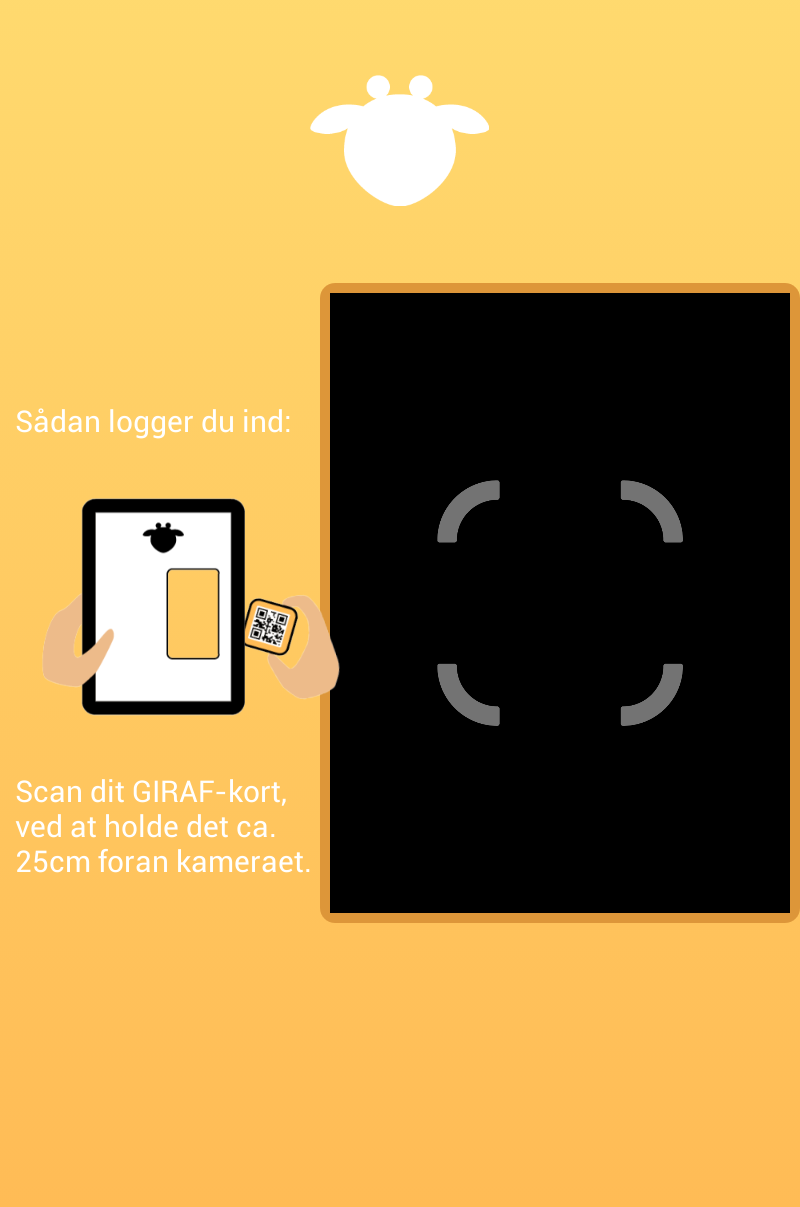
\includegraphics[width=\textwidth, height=3in, keepaspectratio=true] {screenshots-old-giraf/giraf-authenticationactivity.png}
	\caption{\textit{Authentication} activity.}
	\label{fig:launcheractivity:auth}
	\end{subfigure}
	
	\quad % Inserts extra space between rows of subfigures
	
	\begin{subfigure}[b]{.48\textwidth}
	\centering
	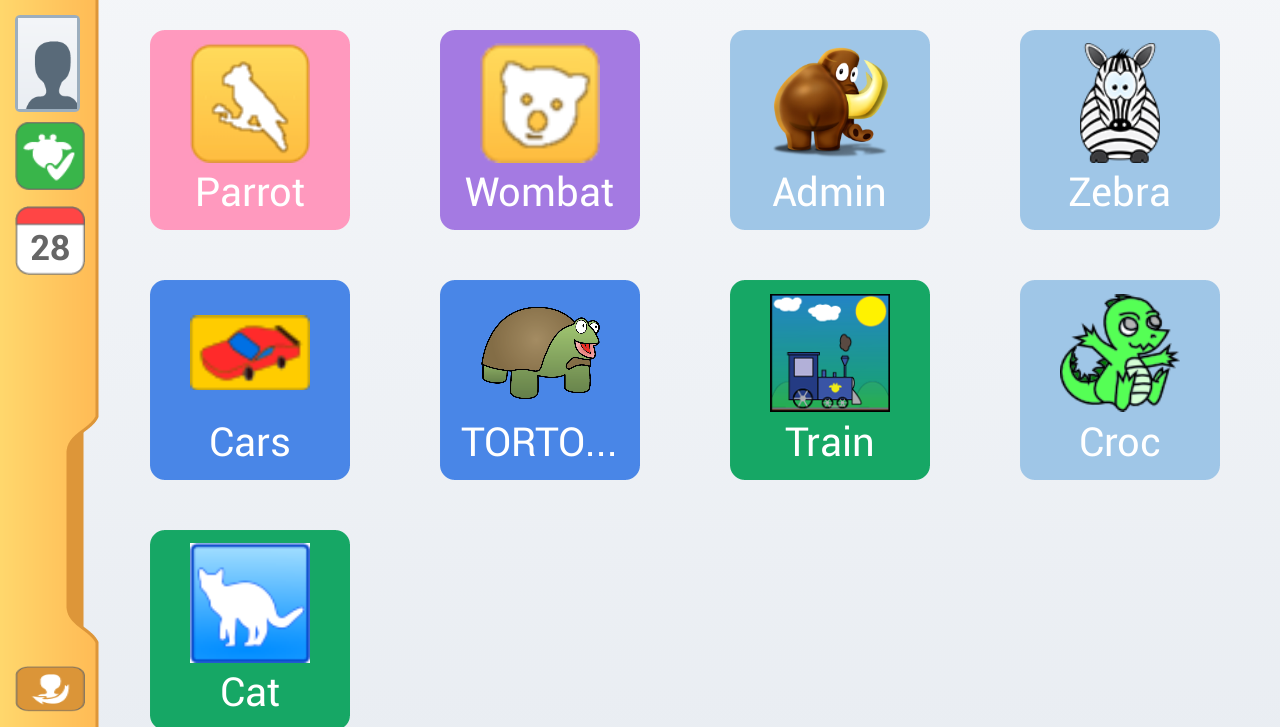
\includegraphics[width=\textwidth]{screenshots-old-giraf/giraf-homeactivity.png}
	\caption{\textit{Home} activity.}
	\label{fig:launcheractivity:home}
	\end{subfigure}
	\begin{subfigure}[b]{.48\textwidth}
	\centering
	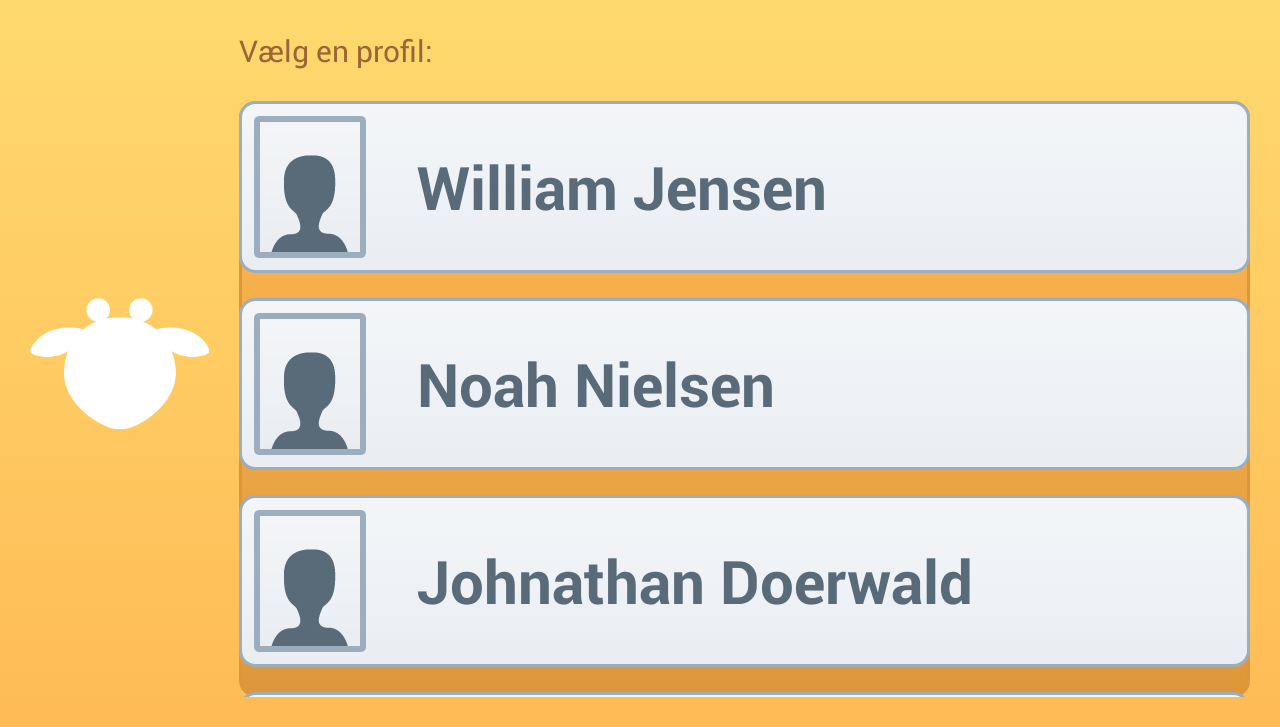
\includegraphics[width=\textwidth]{screenshots-old-giraf/giraf-profileselect.png}
	\caption{\textit{ProfileSelect} activity.}
	\label{fig:launcheractivity:profile}
	\end{subfigure}
\caption{Activities of the \giraf application.}
\label{fig:launcheractivities}
\end{figure}

\paragraph{Logo activity} is not responsible for anything else than showing the \giraf logo for a specified amount of time (as seen in \cref{fig:launcheractivity:logo}), and then redirecting the users to the proper activity.
It redirects to Authentication activity if the user is not logged in, or to the Home activity if the user is already logged in.\thilemann{Discuss if fx activities should be written as inline listings.}

\paragraph{Authentication activity} requires the user to authenticate him- or herself before proceeding. 
\citet{launcher2012} describes how user identification is necessary, as the \giraf settings must be able to vary from user to user. 
The report furthermore describes how autistic children might have problems using a traditional user-name and password system. 
Therefore, the authentication activity is based on a QR-scanner, as seen in \cref{fig:launcheractivity:auth}.
Each child and guardian then uses a small brick with their personal QR-code they scan to identify themselves. 
The activity loads the user information from the database, and proceeds to the Home activity.

\paragraph{Home activity} allows the user to launch \giraf applications available to his or hers user account. 
The availability of an applications depends on whether the application exists locally on that device, and on whether the user is marked in the database as having proper access rights to that application.
The \textit{Home} activity for a test guardian user is seen in \cref{fig:launcheractivity:home} with the user's installed \giraf applicatons.
Furthermore, a number of widgets allows the user to see the synchronization status of the local database in relation to the remote database, and a widget showing current date. 
There is also a button that allows the user to log out, and return to the Authentication activity.
Finally, there is a colour palette hidden in a drawer component, where the user can change the base colour of each installed applications. 
The idea is to make it easier for the children to differentiate between the various applications by being choosing their own colourscheme. 
Ideally the choice of colour should also reflect in the application started from the \launcher, giving the child consistent visual associations throughout \giraf.
The latter is for example implemented in the \textit{Timer} application.\vagner{Add a source to this}\thilemann{Is that necessary?}

\paragraph{Profile Select activity} is started when a guardian launches an application from \launcher. 
It displays a list of all children associated with this guardian (as seen in \cref{fig:launcheractivity:profile}), allowing him or her to choose which child's profile to use when launching the selected application. 
When a child is selected, the application launches, omitting the \textit{Profile Select activity}.
\subsection{Drawer}\label{sec:launcher:drawer}
The drawer is a separate view that is situated in the left-hand side of the \textit{Home} activity.
Its main purpose is to allow \launcher users to apply a new colour-scheme to their installed \giraf applications.

The concept of the drawer is a component that can be shown and hidden at will.
This means that only part of the drawer is visible at all time; it can be dragged towards the centre of the screen to reveal its contents.
Apart from enabling the users to switch colours of their installed \giraf applications, it also contains various informative widgets.
These widgets are a calendar, implemented as \lstinline{GWidgetCalendar}, a server connection indicator, implemented as \lstinline{GWidgetConnectivity}, and a logout button, implemented as \lstinline{GWidgetLogout}.
The implementations of these widgets are a part of \lstinline{GirafComponents}, a separate project in the \giraf system that handles customized Graphical User Interface components.
It should be utilized throughout all \giraf applications to make them look and feel the same.

Illustrations of the drawer in closed and opened positions can be seen in \cref{fig:drawerclosed,fig:draweropened} respectively.

\begin{figure}[h] % Billeder af draweren i åben og lukket tilstand
\centering
	\begin{subfigure}[b]{.48\textwidth}
	\centering
	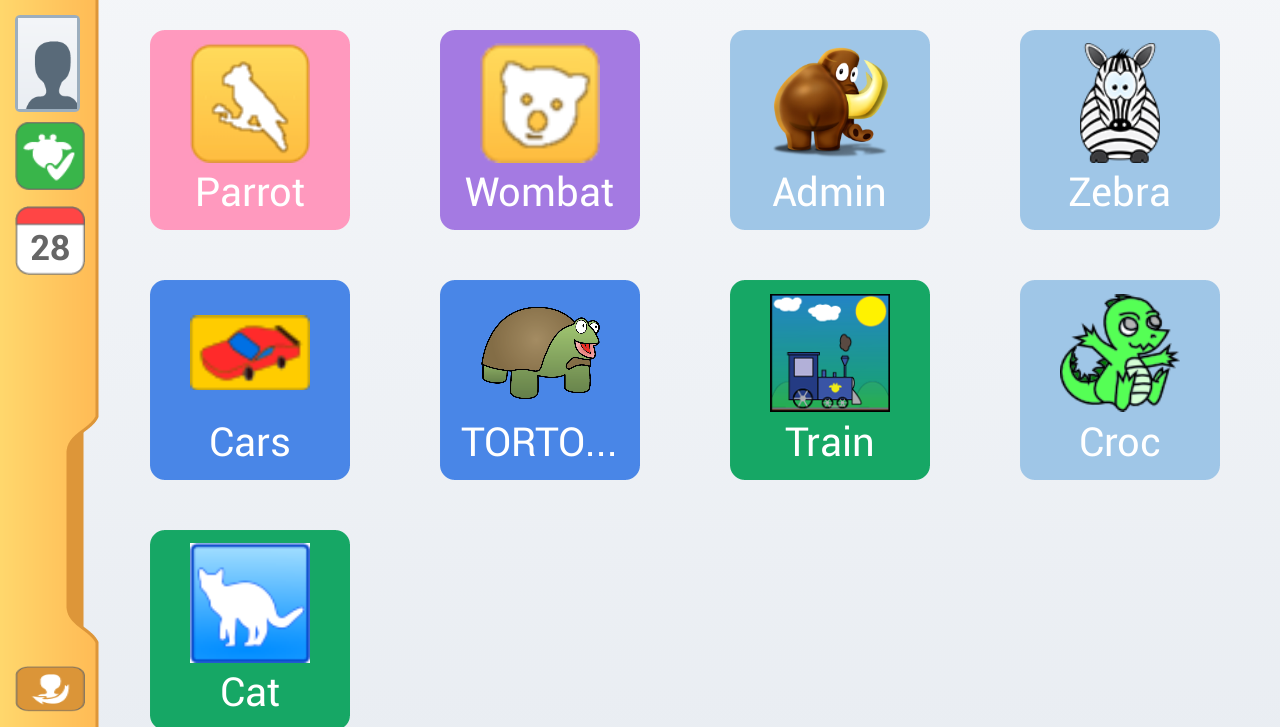
\includegraphics[width=\textwidth]{screenshots-old-giraf/giraf-homeactivity.png}
	\caption{Drawer closed.}
	\label{fig:drawerclosed}
	\end{subfigure}
	\hfill
	\begin{subfigure}[b]{.48\textwidth}
	\centering
	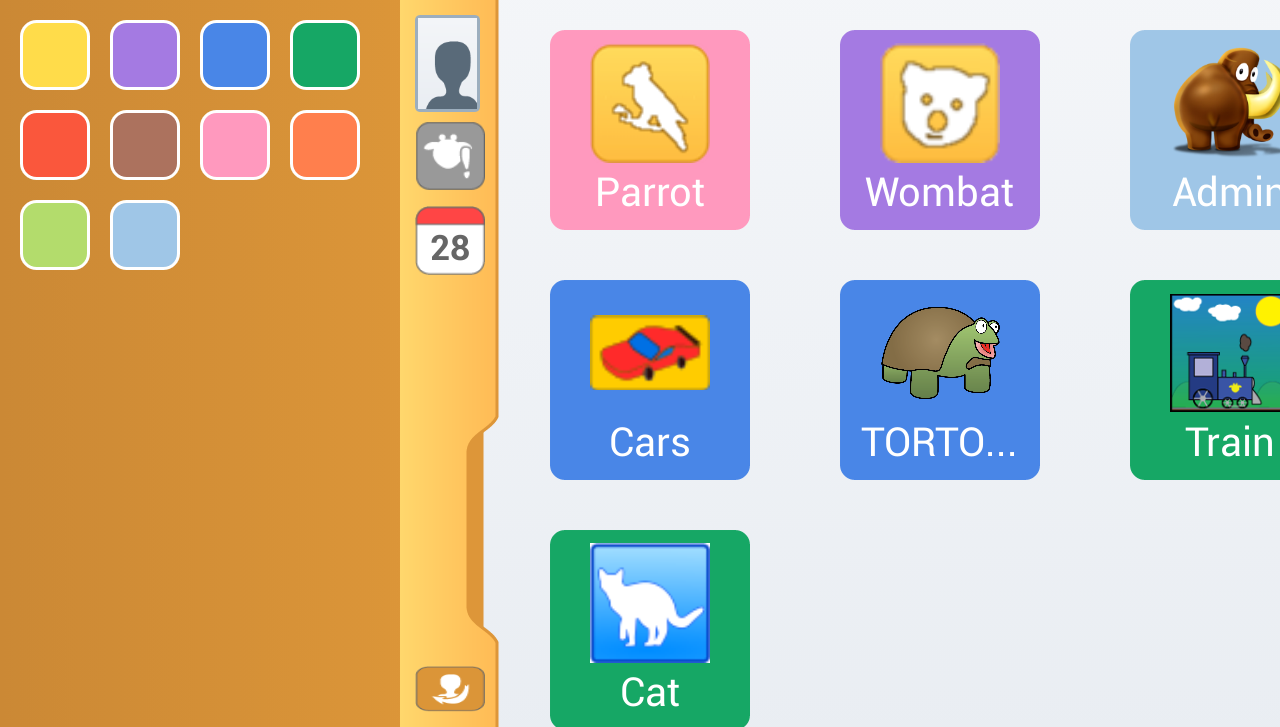
\includegraphics[width=\textwidth]{screenshots-old-giraf/giraf-drawer-fullyextended.png}
	\caption{Drawer fully extended.}
	\label{fig:draweropened}
	\end{subfigure}
\caption{States of the drawer component shown on \textit{Home} activity.}
\label{fig:drawerstates}
\end{figure}

As indicated by \cref{fig:drawerstates}, the drawer already meet the requirement that a colour can be dragged onto an application.
In spite of this, many deficiencies have been located, which are further enlightened by the following sections.

\subsubsection{The Original Drawer}

The original drawer would open by pressing and holding the bar and sliding it to the right.
While being opened, the drawer would push the application icons along with it to the right, resulting in some icons disappearing off-screen to the right.
Furthermore, the drawer would stop when pressure was released from the touch-screen, meaning it could be left in a half-open, half-closed state.
To change the colour of an application, a colour could be drag-and-dropped onto an icon. 
The result would be immediately apparent, as the colour framing the icon would change to the selected colour.

\subsubsection{Desired Improvements}

Since no formal requirements are available and the project group had yet to have a meeting with the customer, the suggested improvements below is based on what we find to be natural requirements of such a User Interface component. 

\begin{itemize}
\item The drawer should be either open or closed. A half-open or half-closed state should result in the drawer popping into the state closest to its current position.
\item The drawer should close while a colour was being dragged, and open again when dropped.
\item The drawer should not push the application icons out of the screen.
\item The source code responsible for the animation of the drawer and the layout of \lstinline{HomeActivity} should be refactored in order to:
\begin{itemize}
\item take advantage of standard Android animations and layout features,
\item allow the activity to dynamically adjust according to display size and
\item reduce the amount of clutter in the source code and improve readability.
\end{itemize}
\end{itemize}

The implementation of the improvements is described in \cref{sec:developments:drawerimprovements}.

\section{Developments}\label{sec:sprint1:developments}
This section considers the problems found in the Analysis and Design (\cref{sec:sprint1:analysis}) of the first sprint.
\vagner{Mention minor bugs, debug mode and focus on home activity, drawer, and restructuring of layout. Also mention functional tests somehow... bare skriv en lille intro}
\subsection{Minor Bugs}

Several minor bugs, anomalies and things that did not work as expected were found in the beginning of the spring.
Considering their negligible significance, we will not discuss them in depth, but rather describe each briefly.

\subsubsection{Child Mode}
Regardless of whether the currently logged in profile is a child or a guardian, \launcher opens the \lstinline{ProfileSelector} before opening an application.
It should only open that activity while using a logged in guardian profile.
The issue is solved by checking on the \lstinline{getRole()} parameter of a profile and then appropriately override the \lstinline{OnClickListener} of the profile selector dialog, depending on the role. 

\subsubsection{Force Landscape Mode}
It is clear from reading previous reports describing \launcher that landscape mode should be forced in all \giraf applications.
Since \launcher is the only application able to enter portrait mode, it is corrected by changing \lstinline{AndroidManifest.xml} to only allow landscape mode for all activities, which contains essential information that is used by the Android system to control its behavior\cite{appManifest}.

\subsubsection{Issues related to other groups}
Two issues caused by other projects are also discovered:

\begin{itemize}
\item The \lstinline{GButton} widget from \textit{GIRAF Components} library crashes any activity that implements it.
\item Danish characters are not encoded correctly in the database.
\end{itemize}

The issues are reported to the groups responsible for these components through our issue tracker, which in effects handles their responsibility over to the other groups.
%\thilemann{Write about the improvements of the launcher}
\thilemann{Maybe also something about refactoring the xml files}
\subsection{Drawer Improvements}\label{sec:developments:drawerimprovements}
As mentioned in \cref{sec:launcher:drawer}, the drawer was opened by pressing and dragging the drawer border.
The code working this animation was based on an \lstinline{OnTouchListener}, focusing mainly on the \lstinline{MotionEvent.ACTION_MOVE} event.
\lstinline{MotionEvent.ACTION_MOVE} would set the position of the entire drawer, panel and bar, to the exact point it had currently been moved to and redraw the elements.
Because the \lstinline{ScrollView} containing the application icons was set to \lstinline{android:layout_toRightOf} in the layout XML files, the \lstinline{ScrollView} would adjust itself to the new position each time the event fired.

The panel of colours was implemented using a \lstinline{GridView} - using the command \lstinline{AppColors.setAdapter(new GColorAdapter(this));}, the \lstinline{GColourAdapter} from \lstinline{OasisLib} would create the correct panel.

Selecting a colour and assigning it to an application worked by means of an \lstinline{OnDragListener} called \lstinline{GAppDragger}.

\subsubsection*{The Improved Drawer}

Opening and closing the improved drawer was implemented with an \lstinline{OnTouchListener} through the \lstinline{MotionEvent.ACTION_DOWN} event and a standard Android \lstinline{TranslateAnimation}.
Pressing the bar fires the event and begins the animation.
A \lstinline{boolean} variable determines whether the drawer was open or closed when the event fired and thus if the animation should translate left or right.
By also adding an \lstinline{OnDragListener} to the drawer, the animation would also play when dragging and dropping colours from the panel; closing the drawer on \lstinline{DragEvent.ACTION_DRAG_STARTED} and opening it again on \lstinline{DragEvent.ACTION_DRAG_ENDED}.

Having the \lstinline{ScrollView} containing the application icons remain static during the animation, was solved by reorganising the source code responsible for the user interface layout. 
Previously, all elements were merely declared in the XML layout file, while positioning of the elements was statically set in the \lstinline{HomeActivity} load code - over 100 lines of parameter setting code.\vagner{maybe not include mocking the previous group?}
This was refactored to have the all positioning declared dynamically depending on screen size, apart from the positioning of the \lstinline{ScrollView}.\vagner{Stefan, write intelligent stuff about dynamic positioning of the ScrollView}
\vagner{Add documentation about the icon indicating opening and closing of the drawer}

The improved drawer fulfils all desired the previously specified requirements, and provides a smoother and more pleasant experience for the user, while refactoring of the acting code provides clarity and readability of developers.\jesper{Is this a little arrogant, considering we haven't actually shown it to users?}\vagner{True, and in sprint 2 we learn that the user doesnt even need the drawer. However, this was what we thought was requirements at the time of writing.}


\subsection{Refactoring the Drawer Layout}
The behaviour of the drawer (as described in \cref{sec:drawer:behaviour}) has the unfortunate effect on the list of applications that it pushes their containing view to the right as the drawer is dragged open.
This is caused by the view (\lstinline|ScrollView|) having the  \lstinline{android:layout_toRightOf} attribute set to be placed to the right of the vertical bar in the layout XML files, which makes its position adjust automatically to the newest rightmost position of the vertical bar each time the bar is moved, effectively pushing the icons of the screen.

The improved implementation includes restructuring all parts of the XML file defining the layout of the home activity, making it adapt to devices with various screen sizes (and pixel density).
Despite of the layout elements not being used correctly and thus not following Android design guidelines, the main issue lies in the fact that many parameters such as heights and widths are set at compile-time through a class containing mostly static fields.
The result is that the layout does not adapt to more than device it has been designed for, which is not viable if the customers, as an example, choose to replace their current devices.

\subsubsection{Restructuring Layout of the Drawer}\label{sec:sidebarlayout:xml}
\jesper{Find a better title. It should not sound exactly like the subsection title.}
To avoid the icons being pushed outside the screen, the layout for the drawer is restructured so its elements are contained within a custom view called \lstinline|DrawerLayout|.
This ensures that the animation and layout hierarchy can be controlled more effectively, making the drawer being drawn on top of other layout elements.
%The custom view is further described in \cref{sec:siebarlayout:java}. % udkommenteret da det refere til en anden udkommenteret section
\Cref{lst:sidebarlayout} shows the elements of the XML layout with most attributes omitted.

\begin{lstlisting}[caption={Structure of the XML layout of the drawer.},label={lst:sidebarlayout}, language=XML]
<dk.aau.cs.giraf.launcher.layoutcontroller.DrawerLayout android:id="@+id/DrawerView" android:layout_marginLeft="-400dp">

<RelativeLayout android:id="@+id/DrawerContentView" android:layout_width="400dp">
<GridView android:id="@+id/appcolors" />
</RelativeLayout>

<RelativeLayout android:id="@+id/SidebarView">
<dk.aau.cs.giraf.gui.GWidgetProfileSelection />
<dk.aau.cs.giraf.gui.GButtonSettings />
<dk.aau.cs.giraf.gui.GWidgetLogout />
</RelativeLayout>

</dk.aau.cs.giraf.launcher.layoutcontroller.DrawerLayout>

<ScrollView android:id="@+id/appScrollView"/>
\end{lstlisting}

Notice the \lstinline|ScrollView| on the last line in \Cref{lst:sidebarlayout}.
The before mentioned \lstinline{android:layout_toRightOf} attribute have been removed, to keep it from being pushed out of the screen.
The negative margin of 400dp defined on line 1 effectively hides the \lstinline|SideBarLayout| when the home activity is just started, revealing only the \lstinline|HomeBar|.
Since the \lstinline|HomeBar| is placed next to the \lstinline|GridView| (in the layout file) with the id of \lstinline!appcolors! and this view has the same width as the negative margin defined on \lstinline|SideBarLayout|, it is the only visible element; giving the impression of a closed drawer.

% \subsubsection{Extending an Android View Class}\label{sec:siebarlayout:java}
% In \cref{lst:sidebarlayout}, the \lstinline|dk.aau.cs.giraf.launcher.layoutcontroller.SideBarLayout| is a reference to the implementation of this class as seen in \cref{lst:sidebarlayout:java}.
% The main reason for not using a \lstinline|RelativeLayout| is that when overriding the \lstinline|onAnimation| methods from the containing activity, is is not being drawn properly, making the drawer flicker when animated.
% Using a custom implementation, it is possible to extend the layout with tailor-made functionality to obtain the desired behaviour.

% \begin{lstlisting}[caption={Extending the Android \lstinline|RelativeLayout| class.},label={lst:sidebarlayout:java}]
% public class SideBarLayout extends RelativeLayout {

%   public boolean isSideBarHidden = true;
  
%   @Override
%   protected void onAnimationStart() {
%     super.onAnimationStart();
%     this.bringToFront();
%   }
  
%   @Override
%   protected void onAnimationEnd() {
%     super.onAnimationEnd();

%     SideBarLayout.LayoutParams params = (SideBarLayout.LayoutParams) this.getLayoutParams();
%     RelativeLayout homeDrawer = (RelativeLayout) findViewById(R.id.HomeDrawer);

%     if (isSideBarHidden) {
%       params.leftMargin = homeDrawer.getLeft();
%       isSideBarHidden = false;
%     } else {
%       params.leftMargin -= homeDrawer.getMeasuredWidth();
%       isSideBarHidden = true;
%     }
%     this.setLayoutParams(params);
%   }
% }
% \end{lstlisting}

% The code (\cref{lst:sidebarlayout:java}) is of trivial character, but makes the implementation of the drawer a lot easier, since it makes it responsible for its placement after animating.
% An Android \lstinline|TranslateAnimation| does not animate the view, but obtains a bitmap of the view which is then animated.
% Without controlling its position after initiating the animation, it would pop back to its original position.
% The position of the \lstinline|SideBarLayout| is set relative to the position of the \lstinline|HomeBar| when \lstinline|onAnimationEnd()| is called.
% \lstinline|this.bringToFront()| simply ensures that the view is rendered on top of other layouts, making it slide on top of them.
% The public field \lstinline|isSideBarHidden| is used to calculating if the drawer should be animated to either opened or closed state.% (as seen in \cref{lst:sidebarlayout:java,lst:draweranimation:homeactivity}).

% \subsubsection{Animating the Drawer}
% The animation of the drawer is started from a touch listener located on the \lstinline|HomeBar| in \lstinline|HomeActivity|.
% \Cref{lst:draweranimation:homeactivity} shows an excerpt of the code that gets called to start the animation.

% \begin{lstlisting}[caption={Excerpt of \lstinline|placeDrawer()| method from the home activity.},label={lst:draweranimation:homeactivity}]
% int to;

% if(mSideBarView.isSideBarHidden)
%     to = mHomeDrawerView.getWidth();
% else
%     to = -mHomeDrawerView.getWidth();

% // Animate the drawer (fromX, toX, fromY, toY)
% TranslateAnimation ta = new TranslateAnimation(0, to, 0, 0);
% ta.setDuration(500);
% if(!mDrawerAnimationRunning){
%   mSideBarView.startAnimation(ta);
%   mDrawerAnimationRunning = true;
% }

% ta.setAnimationListener(new TranslateAnimation.AnimationListener(){
%   @Override
%   public void onAnimationStart(Animation animation){
%     mAppsScrollView.setLeft(mHomeBarView.getWidth());
%   }
%   ...
% });
% \end{lstlisting}

% The member \lstinline|to| is used to decide which direction on the x-axis the view should be animated when instantiating a new \lstinline|TranslateAnimation|.
% Its constructor takes values relative to its current position, which is why all but one parameter is 0.
% The parameter not 0 is the position the animation should animate to on the x-axis.
% Before starting the animation, the left margin of \lstinline|mAppsScrollView| is set to the rightmost position of the \lstinline|HomeBar| to make the \lstinline|ScrollView| stay at its current position.
\subsection{Authentication Activity Error}
When starting \launcher for the first time, the application crashed and threw an \lstinline{OutOfMemoryError} when reaching the \authenticationactivity.
The core of this problem is caused by an animation in the activity, implemented as an instance of the Android class \lstinline{AnimationDrawable} -- a class designed to create animations from a sequence of images.
According to the Android documentation \citet{androidreference}, the implementation is technically correct, but it is found that when an instance of \lstinline{AnimationDrawable} is created, it loads the entire sequence of images into main memory of the device at once.
The images are contained within the application in the compressed Portable Network Graphics (PNG) format.
However, as they are loaded, Android converts each image to a 32-bit bitmap, which is 4 bytes per pixel, making the images take up about 20 times the space, thus resulting in the animation using about 40 MB of memory. 
We hypothesized that this was the source of the \lstinline{OutOfMemoryError}.

One solution to this problem is to create a new class which simulates the behaviour of \lstinline{AnimationDrawable}.

By simulating \lstinline{AnimationDrawable}, we only keep one image in memory at all times and avoid the error.
This is achieved by a recursive method, which is changing the shown image automatically.
The images are stored in a static array which is iterated repeatedly using the method \lstinline|postDelayed()| which is possible to run code after a set amount of time.

\begin{lstlisting}[caption={Improved implementation of handling the animation.},label={lst:methodPlay}]
private void play(final int pFrameNo){
  mImageView.postDelayed(new Runnable(){
    @Override
    public void run() {                    
      mImageView.setImageResource(mFrames[pFrameNo]);

      if(pFrameNo == mLastFrameNo)
        play(0);
      else
        play(pFrameNo + 1);
    }
  }, mDuration);
}        
\end{lstlisting}

\section{Functional Tests}\label{sec:sprint1:testing}
As one of our goals is to increase the reliability of \launcher, we decided to conduct functional testing on the application.
We studied the specifications formulated by the earlier development teams in \citet{launcher2011,launcher2012}, and then studied how well \launcher correspond to these specifications, by using the program in a number of different ways. 

Furthermore, a number of test cases are not directly derived from the old specifications, but from what we find reasonable to expect of the application, based on our own knowledge of the system.

The tests described here are performed by operating the running application, and are explicitly not based on our knowledge of the source code. 
This characterizes our tests as being dynamic black box testing. 

A number of test cases that would have been relevant, is not performed in this sprint as we deem that they not sufficiently interesting, considering the time needed to run them. This includes using \launcher with a varying set of applications and children.
These test cases require significant changes to the test data hard coded into the \giraf system, or repeatedly installing and uninstalling applications from the device.
As there is currently no central repository of stable application builds, most of the time would be spent building, installing and resetting different applications.

We only describe the results we find the most interesting in this section; mainly tests that failed in a significant way.

\subsection{Specifications}
In the 2011 report by \citet{launcher2011}, the following specification for \launcher is presented:

\begin{quote}
\begin{itemize}
	\item \textit{List only applications that is part of the \giraf system.}
	\item \textit{List only applications that the user is able to use, according to the user's capabilities.}
	\item \textit{List only applications if their usage is not limited by the current location or time.}
	\item \textit{Only display application names if the user is able to read.}
\end{itemize}
\end{quote}

Common to all these, is that they are either difficult to test, or simply not implemented (some may have been to some degree in 2011, but then removed by the 2012 team).
The difficulty stems from the necessity of manipulating test data, that is hard coded into the local database of each device. 
We decided it would be more reasonable to revisit these test cases when \giraf's database system is ready for use.

The 2012 report by \citet{launcher2012} contains no explicit specifications, but does contain a list of use cases. 
These form the basis of our tests:

\begin{quote}
\begin{itemize}
	\item \textit{New guardian log in.}
	\item \textit{Configuring an application for a child.}
	\item \textit{Launching an application for a child in guardian mode.}
	\item \textit{Letting a child use an application for a limited time.}
\end{itemize}
\end{quote}

Note that their report also contains an explanation of each use case. 
We leave these out for brevity.

\subsection{Test Results}\label{sec:sprint1:testing_results}
Below is shown a selection of our test cases and their results.
As mentioned in the introduction of this section, we will only discuss the most interesting results, i.e. tests that led to the discovery of significant issues.

\subsubsection{Changing the Colour of an Application Icon}

\paragraph{Specification:} Configuring an application for a citizen.
\paragraph{Test case:} Use the drawer to change the colour of an application, and check if the change is applied to both the application's icon, and its own user interface.
\paragraph{Result:} The colour of the icon changed immediately, but when starting the application, it still used the pre-change colour. 
A little experimenting showed that the change is not applied to the application until the user logs into \launcher again.
\paragraph{Resolution:} The issue was resolved, and the change in colour is now reflected in the application immediately.

\subsubsection{Applications that Crash Launcher}

\paragraph{Specification:} Starting an application for a citizen in guardian mode.
\paragraph{Test case:} Open an application with a randomly selected citizen profile by using the profile selector.
\paragraph{Result:} While not directly related to the intent of the use case, during the test, we attempted to open what turned out to be a non-working version of a \giraf application. 
The application suffered from an unhandled exception, causing both it and \launcher to crash. 
This is not satisfactory, as \launcher should always work on top of the device operating system, denying the citizen access to device settings when using the device without supervision.
\paragraph{Resolution:} The issue was resolved by making \launcher catch all exceptions thrown by the \giraf applications it hosts.

\subsubsection{Use of Device Buttons}

\paragraph{Specification:} The device buttons (\textit{Back}, \textit{Home}, and \textit{Multitasking}) should have no effect in \mainactivity and \authenticationactivity, as the user should not be able to ``back out'' of \launcher to the device OS.
\paragraph{Test case:} Use the device buttons in different activities and situations.
\paragraph{Result:} In both \mainactivity and \authenticationactivity, applying the \textit{Home} and \textit{Back} buttons made \launcher restart. 
The \textit{Multitasking} button always activates the multitasking screen of the device OS.
\paragraph{Resolution:} The \textit{Back} button are suppressed by overriding a listener method.
We were unable to find similar means for suppressing the other two buttons, as we unsuccessfully returned to this issue in the second sprint, as described in \cref{sec:sprint2:backlog}.

\section{Sprint Summary}\label{sec:sprint1:review}
\subsection{Evaluation}
Overall, the first sprint was a success for us.
All task were finished and \launcher is now ready for the sprint review together with the clients, receiving feedback regarding the next steps.

However, for various reasons, the meeting does not yield the desired results for planning the next sprint.
Therefore, the groups decide to appoint a single person responsible for planning and executing this meeting in the future.
The chosen person is from this group, so the details of this and later sprint reviews are discussed in depth in \cref{sec:collab:sprintend}.

\subsection{Backlog}
As mentioned above we did not get any feedback during the sprint review to use for planning our next sprint.
We still think there are elements to improve in \launcher, but we cannot immediately continue the development, before having explored whether the clients have further requirements for the application.
These are explored in \cref{sec:sprint2:overview}.
\chapter{Second Sprint}\label{chap:sprint2}

\section{Sprint Overview}\label{sec:sprint2:overview}
As the described in \cref{sec:sprint1:review}, the end of the first sprint left us unsure of whether there was more work to be done on \launcher, and if so, what this work could be. 
We decide that it is necessary to arrange a meeting with some of the clients, in part to hear their thoughts on the current version of \launcher, and in part to discover new features.
During the first sprint we informally discussed ideas for new features.
These features include an improved format for the profile selector, and a new Settings application, providing a uniform interface for changing settings across all applications. 
To provide a good foundation for presenting and discussing these ideas with the customers, we design a number of prototype drawings of how our ideas could be realized.

A separate important issue in this sprint is adapting \launcher for new versions its dependencies. 
The \textit{OasisLib} library underwent drastic changes at the end of the first sprint, which unfortunately resulted in several applications, including \launcher, being unable to run.

In summary, the main points of this sprint are:

\begin{itemize}
\item Description of the designed prototypes in \cref{sec:sprint2:analysis}, with summaries of the first meeting in \cref{sec:sprint2:firstmeeting} and the second meeting in \cref{sec:sprint2:secondmeeting}.
\item Description of the migration to the new OasisLib in \cref{sec:sprint2:developments}
\end{itemize}\vagner{Is this seriously all we did?}

\section{Analysis and Design}\label{sec:sprint2:analysis}
Intro here...
\subsection{Prototypes}\label{sec:sprint2:prototypes}

At the end of first sprint, the existing features of \launcher were polished and the project would only need to be kept updated with the implementation of the database. \vagner{Verify that this is indeed what actually happened}
However, the review meeting of sprint one determined that it was desired for launcher to possibly have additional features:

\begin{itemize}
\item Selection of profiles might be desired to be selectable elsewhere in \launcher without starting an application.
\item Settings for different applications could be set from an activity accessed from \launcher.
\item Specification of which applications different users can access could likewise be set from and accessed from \launcher.
\end{itemize}

It was decided to have a brainstorm to gather ideas regarding these features, create prototypes of the best ones\footnote{The prototypes regarded as being the best, were deemed so by the project group.} and present these to the customers for feedback.

The prototypes created were \textbf{low fidelity, horizontal} prototypes, as described in \citet[p. 184-195]{debBook}, made partly with screenshots of existing functionality and partly with the modelling tool Gliffy (\citet{gliffy}).
The purpose was to convey several different ways of including the above features, while not spending too much time creating them.

\subsubsection{Profile Selection}

At the end of sprint one, the profile selection would only appear when launching an application, as illustrated by the state chart diagram in \Cref{fig:statechartProfileSelectorInitial}.
\insertfigure{width=\textwidth}{statechartProfileSelectorInitial}{State chart diagram for the original process of choosing a profile.}{fig:statechartProfileSelectorInitial}
Two alternatives where suggested:
\begin{itemize}
\item Selection of a different profile from within \launcher.
This would work by pressing the profile picture, giving a list of profiles to choose from.
Being relevant only for a guardian, the profiles selectable should only be the guardian itself and the child related to him or her.

\item Selection of a different profile from within each individual application.
While this solution does not require any modification of \launcher, it was a favourable option.
Each application would then have its own profile selection button to initiate the activities
\end{itemize}

Common for both alternatives was to display the currently selected profile in the top of the pane.
Illustrations can be seen on \Cref{fig:profileselectionlauncherdropdown,fig:profileselectionapppopup} respectively. For an explanation of the suggested process of choosing a profile see the state chart diagram in \Cref{fig:statechartProfileSelectorBubble}.

\begin{figure}[h] % Billeder af profile selector
\centering
    \begin{subfigure}[t]{.48\textwidth}
    \centering
    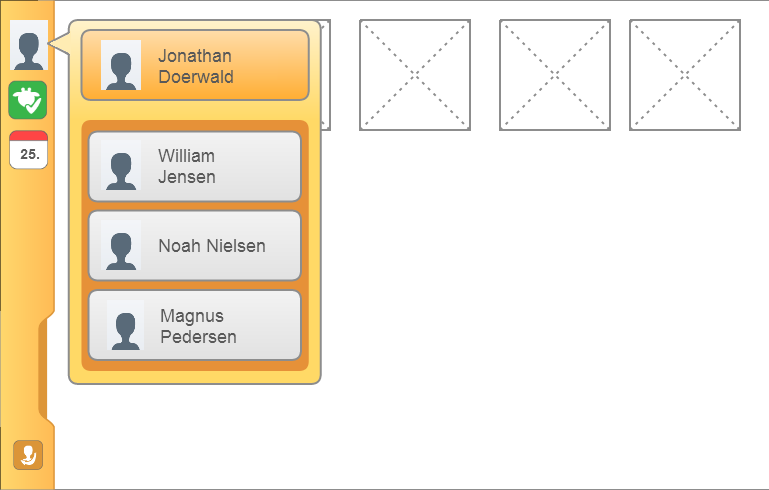
\includegraphics[width=\textwidth]{sprint2/profileselectionhomescreen-dropdown}
    \caption{The dropdown profile selection option. This would appear when tapping ones profile picture as a guardian.}
    \label{fig:profileselectionlauncherdropdown}
    \end{subfigure}
    \hfill
    \begin{subfigure}[t]{.48\textwidth}
    \centering
    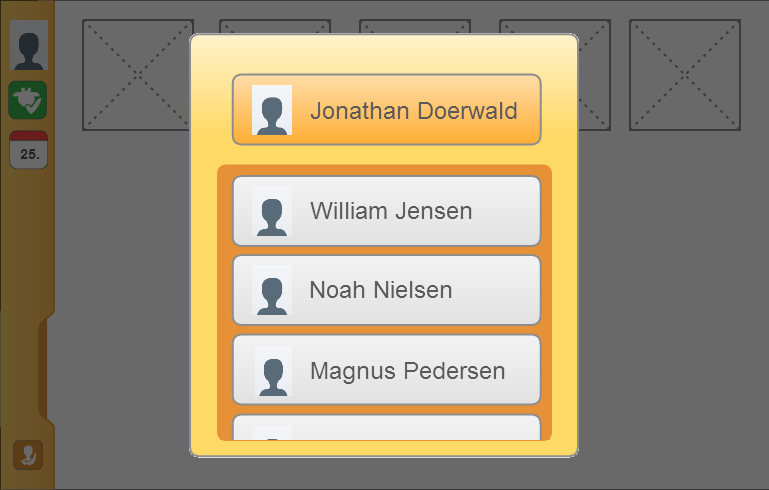
\includegraphics[width=\textwidth]{sprint2/profileselection-dialog-finish}
    \caption{The profile selection pop up. These would only appear while pressing the appropriate button while inside an application.}
    \label{fig:profileselectionapppopup}
    \end{subfigure}\\
    \begin{center}
    \begin{subfigure}[t]{1\textwidth}
    \includegraphics[width=\textwidth]{figures/statechartProfileSelectorBubble.tikz}
    \caption{State chart diagram for the suggested alternative process of choosing a profile.}
    \label{fig:statechartProfileSelectorBubble}
    \end{subfigure}
    \end{center}

\caption{Suggestions for the new profile selector.}
\label{fig:drawerstates}
\end{figure}

\subsubsection{Settings}

At the end of first sprint, settings for different applications where handled inside those applications exclusively.
The idea of centralizing the settings for the different applications was formed both to streamline data for the database, but also to grant the user a better overview over the settings shared by applications.

Again, two alternatives were presented:
\begin{itemize}
\item A settings activity, accessible from \launcher only.
This activity would contain settings for all applications enabled for the selected user, as well as selecting which applications should be enabled for that profile.
This would also include the native Android settings.
\item Letting each application have a settings button.
This would preserve the current setup.
\end{itemize}

The first option is the most encompassing one, containing functionality for both manipulate settings for other applications and decide which applications can be used with different users.
It was furthermore discussed to add functionality, allowing the user to add applications from Google Play to \launcher.
The settings part of the settings activity can be seen in \Cref{fig:settingsprototype}, while the application management part can be seen in \Cref{fig:appsmanagement}.

The second option is more centred on making the settings screen streamlined across applications and would thus be a operative project with the GUI project group.
An example of settings for \launcher can be seen in \Cref{fig:appsettingsprototype}.

\begin{figure}[h] % Billeder af draweren i �ben og lukket tilstand
\centering
    \begin{subfigure}[t]{.48\textwidth}
    \centering
    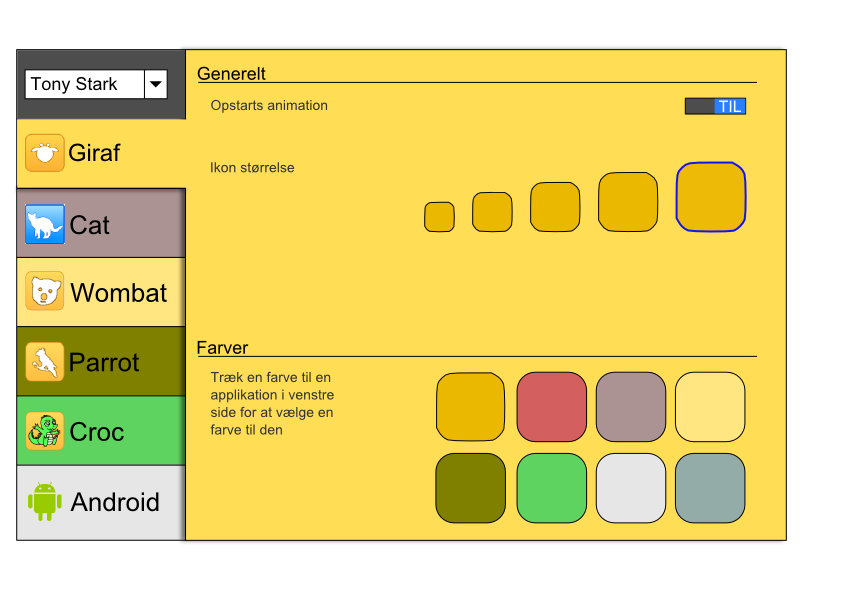
\includegraphics[width=\textwidth]{sprint2/settings}
    \caption{The settings manipulation part of the settings application. in this example, settings for \launcher can be seen. The current profile being edited can be seen in the top left corner.}
    \label{fig:settingsprototype}
    \end{subfigure}
    \hfill
    \begin{subfigure}[t]{.48\textwidth}
    \centering
    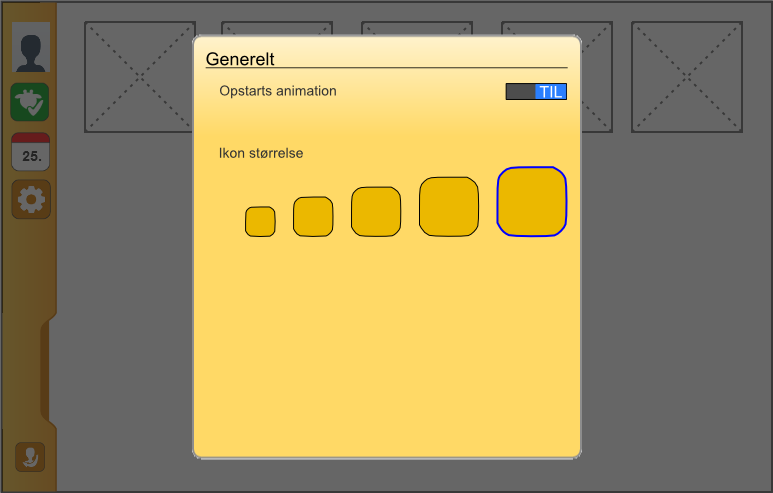
\includegraphics[width=\textwidth]{sprint2/settings-dialog}
    \caption{The settings for a single application. In this example, the settings for \launcher can be seen.}
    \label{fig:appsettingsprototype}
    \end{subfigure}\\
    \begin{subfigure}[t]{.48\textwidth}
    \centering
    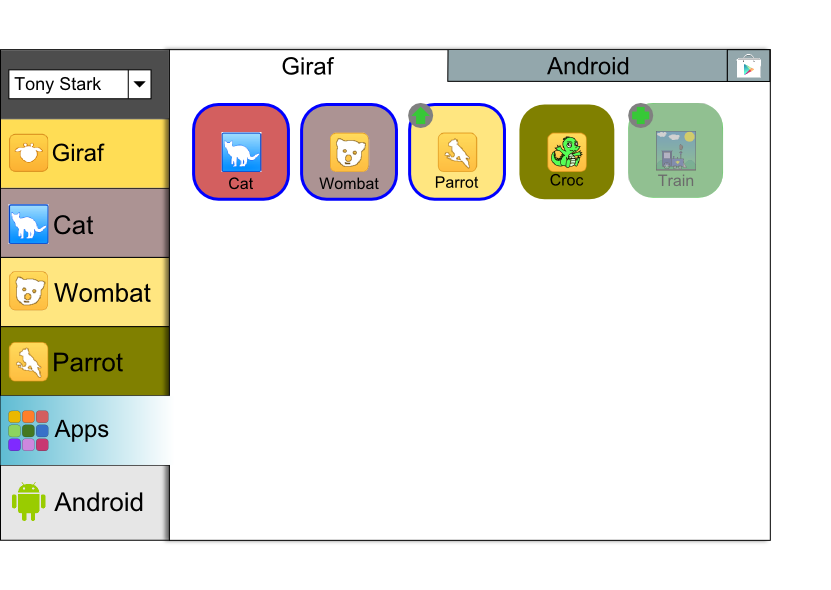
\includegraphics[width=\textwidth]{sprint2/apps-colorexperiment}
    \caption{The application management part of the settings application. \giraf or Android (Google Play) applications can be chosen in the pane in the top. The current profile being edited can be seen in the top left corner.}
    \label{fig:appsmanagement}
    \end{subfigure}
\caption{Suggestions for settings and application management.}
\label{fig:drawerstates}
\end{figure}

\subsubsection{Profile Info}
\frederik{Maaske vi skal undlade denne section, kunderne var ikke vilde med det.}
The group had an idea of displaying information about the user currently logged in in the drawer section of \launcher.
This is a relatively small feature that would be trivial to implement.
An example can be seen in \Cref{fig:profileinfo}.

\insertfigure{width=0.48\textwidth}{sprint2/profil-info}{An example of information about a user seen in the drawer.}{fig:profileinfo}
\section{First Customer Meeting}\label{sec:sprint2:firstmeeting}
This section focuses on the first customer meeting that was held to determine the viability of the thoughts described in \cref{sec:sprint2:prototypes}.

It was held together with one customer and an external contact on the 1st of April, 2014.
The customer is Drazenko Banjak from the institution called Egebakken, which is a school for children with autism.
The external contact is Pernille Hansen Krogh, the owner of a company called Mymo, which works with design and decor optimized for learning.\footnote{In plural they are referred to as \textit{customers}.}


\subsection{Feedback}\label{sec:firstmeeting:feedback}
Since the contents of the meeting mostly concerned new developments, a slide show was made to support the presentation of the prototypes.
Following that the customers not staying to discuss \giraf at the status meeting, a tablet with the most recent version of \launcher was also brought to get feedback on the changes made during the first sprint (\cref{chap:sprint1}).


\subsubsection{Profile Selector}
The profile selector prototypes (\cref{fig:profileselectionlauncherdropdown,fig:profileselectionapppopup}) was presented, and both customers were thrilled about the idea of being able to easily switch profiles from \launcher and each \giraf application individually.
The design was by Pernille considered as being ``clean and intuitive'', as outlined in \cref{appendix:firstmeeting}.


\subsubsection{Settings}
The idea of adding settings management to \launcher, both regarding settings for \launcher itself and for all \giraf applications, was the main idea to be assessed at these meetings.
Therefore the two possibilities as seen in \cref{fig:settingsprototype,fig:appsettingsprototype} were presented.
The customers liked the visual look of the prototypes, but had a big concern that the design would add to much complexity to \launcher and that Drazenko's colleagues at Egebakken would be scared of using it.
They liked the idea of changing settings from each application for the logged in user, even though we argued that it would impose higher workloads to the guardians if they need to change settings for many users.
A hybrid consisting of both possibilities were suggested to overcome this.

The customers made the following suggestions based on the presentation of the settings management application:

\begin{itemize}
\item Add an external (Android) application to \launcher.
\item Restrict access to use other applications on a per-user basis when it's guardian has assigned a child to work with a specific application.
\end{itemize}

These suggestions are further considered in \cref{chap:sprint3}.


\subsection{Clarification of Issues}
Although \cref{sec:launcher:drawer} consider improvements to the drawer component in \giraf, a major discussion at the meeting was about whether to keep the drawer or not.
More specifically, Pernille made us rethink if users should be able to colour applications.
If not, it will render the drawer unnecessary.

To overcome this decision, Pernille also suggested us to hold another meeting with Birken, since they are the originator of the requirement.
This is discussed further in \cref{sec:sprint2:secondmeeting}.

\subsection{Communication}
At this meeting the communication between the customers and us were quickly characterized as being problematic.
The reason being that one customer did not always quite understand what we were asking for.
The group establishes two possible reasons:
(1) He (Drazenko) is lacking technical domain knowledge and does not know the correct terminology\footnote{We quickly established this fact and thus made an effort to use as many non-technical terms as possible.} and (2) He is of foreign extraction and is thus not a profound speaker of Danish.
Pernille on the other hand showed great technical understanding even though she, as an external contact, had no previous knowledge of the \giraf project.
Thus, she did not contribute regarding how \giraf is used 'out in the field', but touched areas that made us rethink previous decisions.

The above facts resulted in a somewhat vague feedback, in the sense of the customer not always being able to clearly formulate his requirements.
Another problem was that when asking a question one topic, feedback was given on another topic which might be irrelevant in the context of \launcher.

Because of these defects in communication, the meeting is not considered to be a success.
\section{Second Customer Meeting}\label{sec:sprint2:secondmeeting}
\thilemann[inline]{Add a reference to the customer meeting in appendix - something like done in the preceeding section...}
The meeting was held the 3rd of April 2014 with two representatives Mette Als Andreasen and Kristine Niss Henriksen from the nursery for children with ASD, called Birken.
The same prototypes was presented as those in the previous meeting (\cref{sec:sprint2:firstmeeting}).
The main purpose of the meeting was to get feedback from a customer that we had not received feedback from before, while also inquiring about some conflicting requirements of this particular customer.

\subsection{Feedback}\vagner{This feedback is based on the presented prototypes, and so, the prototypes described as presented in the section about prototypes, should match these}
The customer was excited about the presented prototypes.

\subsubsection*{Profile Switcher}
The profile selection tool was preferred as a combination of the two options -- as a selector inside each launched application and as a tool-tip from clicking the profile picture in \launcher.

\subsubsection*{Settings}
The settings tool was preferred also as a combination.
Accessing the settings related to each application from inside that particular application was the most important of the two. Accessing the settings is achieved pressing a button with an image of a gear.
Furthermore, pressing the settings button while in \launcher should open a full-screen activity, where settings for both \launcher itself and all installed applications could be manipulated.
An important aspect of the settings was the ability to copy settings from one user to another.

\subsubsection*{External (Android) applications}
Lastly, the idea of being able to add applications through \launcher was well received, including applications from Google Play.
The customer especially liked the idea of enabling applications on a `per user' - basis.
This functionality was advised to be in the settings activity found in \launcher.

\subsubsection*{Android buttons}
Apart form the prototype, the solution of overriding the ``Home'', ``Back'' and ``Multitasking'' buttons was accepted, but the customer preferred it to be disabled completely.
It was suggested by the customer to utilized the Android equivalent of iOS' `Restricted Access'', to achieve the preferred result.

\subsection{Clarification of Issues}
One mayor issue regarding conflicting requirements was clarified at this meeting.
Previously, there as a requirement of a black-and-white colour scheme, but also a requirement of changing colours.
It was then clarified that this requirement was related only to the pictograms and not to the program as a whole, meaning the pictogram should in general be black and white and those in colour should be able to converted to black and white.
The drawer functionality in \launcher of changing the colour of applications was not a requirement and not particularly important for the customer.

\subsection{Communication}
Communication with this customer was more smooth than at the previous meeting, however, there was still comprehension barriers.
Most barriers were related to the customer not understanding what features would be trivial to implement and which would be exceedingly difficult.
Furthermore, questions asked by the group would often have to be reformulated for the customer to understand it completely.
However, the customer often explained how each question was understood, and always pointed out elements they did not understand.
This aided greatly when there were communication problems.

This customer furthermore expressed more concretely what was desired from the application.
Additional questions from the group were still required, but were answered to completion with references to desires.

Overall, the meeting was regarded as a success, with constructive feedback.


\section{Sprint Summary}\label{sec:sprint2:review}
Remember to write sprint review \vagner{Dette er min section!}

\chapter{Third Sprint}\label{chap:sprint3}

\section{Sprint Overview}
The customers feedback to the prototypes in the second sprint provided vital information about the important parts of the settings, which gives a complete overview of how the settings should be implemented.
This sprint is mainly focusing on the implementation of settings to \launcher.

\section{Analysis and Design}
Here  the sections regarding analysis and design in this sprint will be included.\vagner{once we are done with this section, we should add more introductions}

\subsection{Disabling the Drawer}
As described in \cref{sec:sprint2:firstmeeting,sec:sprint2:secondmeeting}, the purpose of the drawer is founded in a misinterpretation.
It was thought as being important to be able to colour the each \giraf applications accessible from \launcher.
However, at the meeting, it was clarified no such requirements for the applications exist;
what the customers want is to switch the colours of \textit{pictograms}, being able to also show them in black and white, since some citizens handle coloured pictures better than black and white ones and vice versa.\\

Some additional problems are found with the drawer.
These are mostly centred upon other applications absorbing the colour given to them by \launcher, and using that as their main theme.
However, this means that for each possible colour the \launcher can give an application, it needs to implement a colour scheme that fits with the given colour.
This is especially a problem for applications using a wide variety of colours.\\

Since the purpose of the drawer is not a requirement per se, and the colouring functionality caused problems in other applications, it is decided to disable the drawer since it serves no particular purpose.
In effect, the code for animating the drawer remains as is, in case the functionality at a later time will prove useful.
This way, should a future group need to implement the drawer, they merely have to uncomment part of the code.
\subsection{The Settings Library}
The idea behind the settings library was to create a streamlined and uniform user interface for changing settings across the entire \giraf project. As discussed in \jesper{Indsæt ref til kundemøde 2}, we agreed with the clients that settings should accessible through two methods:
\begin{itemize}
	\item A dialogue box in each individual application, containing only settings relevant to that specific application. The dialogue box should be displayed when the user presses a button that is identical throughout all \giraf applications, making it easier for users to find.
	\item A unified settings activity, where the user has immediate access to all settings for all \giraf applications. This activity should be a part of the Launcher. Besides the settings of the individual applications, it should also contain relevant settings pertaining to the user, e.g. which applications the user should be allowed access to.
\end{itemize}

It is immediately apparent that for making both these approaches work concurrently, we would need to create a single plan for how user settings should be handled throughout the \giraf project. In the following we will describe this plan.

\subsubsection{Concept}
We decided that the entire system should consist of four components, to be implemented separately:
\begin{itemize}
	\item The unified settings activity should be implemented as a part of the Launcher, and therefore the implementation of this component naturally falls to ourselves. Excluded from this task is the settings of the individual applications.
	\item A dialogue box able to contain the settings for an arbitrary \giraf application. Included in this is a standard button for launching the dialogue box. As this is user interface component useful to all applications, it should be implemented by the group responsible for the \giraf GUI library.
	\item A set of settings for each \giraf applications. As these sets may vary widely in content and complexity from application to application, and furthermore may change along with their associated applications over time, these should be defined and implemented by the individual project groups. 
	\item A method for storing the settings in the database, allowing the users to easily use the same settings across several devices. This should be implemented by the database group. 
\end{itemize}

\subsubsection{Technical Design}
The big challenge of implementing the above concept, is how to allow the settings interface layout of each application to also be used in the unified settings activity. 

Our initial idea was to ask each group to create a fragment with their settings layout within their own activity, which our settings activity would then be able to load into the unified settings activity. This would isolate the responsibilities of each group, and keep overall complexity to a minimum. However, after some research it turns out that sharing fragments across applications is an ``unnatural'' operation in Android\frederik{Readthrough make real explanations find source.}. While possible, it is not very elegant, even when only sharing a single fragment between two applications, and it results in considerable complexity when scaled to our needs.\frederik{Hvordan var det præcis det virkede?} To simplify this, \launcher could include all other projects as dependencies when compiling, but this would have made the \launcher project unnecessary bloated and difficult to work with.

Another possibility was make the individual applications implement an interface, where a function would add the application's setting-widgets to a given view. While Android provides facilities for inter-application communication through its \textit{Broadcast} mechanism\jesper{indsæt cite}, this requires all the involved applications to be running. This is not an acceptable condition in this situation. 

We finally decided on creating a common settings library, to which all groups added a layout fragment for their own application. This library should then be included with every project that contributes to it, so they can read their own settings from it, and to \launcher, which can use the layouts for the settings activity. This requires a single project to which all developers on the \giraf project have write access, which makes it hard to manage, but it is on the other hand the simplest technical solution. A concrete disadvantage is that errors in the various settings fragments will influence \launcher, but our group will have complete authority over the settings library project, and have the right to make changes necessary to allow \launcher to compile and execute. 

\subsection{Adding Settings to \giraf}\label{sec:sprint3:designsettings}
The idea behind providing a way to change settings from \launcher for both itself, but also other \giraf applications, is to create a streamlined and uniform user interface for changing settings across the entire project.
This section discusses how to design the architecture of what will be an activity implemented in the context of \launcher, to contain the settings.

\subsubsection{Choosing Between Prototypes}
As discussed in \cref{sec:sprint2:secondmeeting}, the customers agreed that settings should be accessible through two methods:

\begin{itemize}
	\item A dialogue box in each individual application, containing only settings relevant to that specific application (as seen in \cref{fig:appsettingsprototype}). 
	The dialogue box should be displayed when the user presses a button identical throughout all \giraf applications, making it easier for users to find.
	\item A unified settings activity, where the user has immediate access to all settings for all \giraf applications, which should be a part of the \launcher. 
	Besides settings of individual applications, it should also contain settings available to a per-user basis, e.g. which applications the user should be allowed access to.
\end{itemize}

It is immediately apparent that for making both these approaches work in parallel, a single plan for how user settings are handled throughout the \giraf project is needed. 
In the following paragraph this plan is described.

\paragraph{Concept}
It is decided that the settings system should consist of four components, to be implemented separately:

\begin{itemize}
	\item The unified settings activity should be implemented as a part of \launcher, and therefore the implementation of this component naturally falls to ourselves. 
	Excluded from this task is the settings of the individual applications.
	\item A dialogue box able to contain the settings for an arbitrary \giraf application. Included in this is a standard button for launching the dialogue box. 
	As this User Interface component is useful to all applications, it should be implemented by the group responsible for the \giraf GUI library.
	\item A set of settings for each \giraf application.
	As these sets may vary widely in content and complexity from application to application, and furthermore may change along with their associated applications over time, these should be defined and implemented by the individual project groups. 
	\item A method for storing the settings in the database, allowing the users to easily use the same settings across several devices. This should be implemented by the group responsible for the remote database (As this group has other priorities, the settings will initially be saved locally on each device).
\end{itemize}

\paragraph{The challenge with Implementing Settings} using the above concepts is how to allow applications other than \launcher to access the settings User Interface running in the context of \launcher as an activity.

\begin{itemize}
\item 
The first option is to ask each project group to create a \lstinline|Fragment|, which the settings activity in \launcher should be able to open.
This approach will isolate the responsibilities of each group and keep the overall complexity to a minimum.\thilemann{Why? Where to put the files and what about git? Project dependencies?}
Although there is an official way for loading a custom class\cite{customClassLoading}, it is complex and it will make the coupling of \launcher and other applications very tight.\thilemann{Does class loading even solve this???}
Additionally it is difficult to make the loading of custom classes dynamic, since the name of the class to be loaded has to be known.
The method of custom class loading is intended to be used when a project exceeds 64.000 method references, which is the limit of the Dalvik Virtual Machine.
Each Android application is running as an instance of Dalvik that sandboxes the data of the application, making it impossible for other to access it.

\thilemann{To simplify this - meaning what?}
To simplify this, \launcher has to include all other projects as dependencies when compiling, which will make the \launcher project unnecessary bloated and difficult to work with.

\item
Another possibility is to make the individual applications implement an interface, where a function would add the application's setting-widgets to a given view.
While Android provides facilities for inter-application communication through its \textit{Broadcast} mechanism\cite{broadcastReceiver}, this requires all the involved applications to be running.
This is not an acceptable condition in this situation. 
\end{itemize}
 
\subsubsection{The Final Design}
Instead of the to presented options above, another design is chosen.
An Android feature called Intent Filters allows applications to request an action from another Android component; an activity, a broadcast receiver, a content provider or a service.
It is implemented by adding \lstinline|<intent-filter>...</intent-filter>| to the Android Manifest with its actions (or intentions) defied within.\cite{intentFilter}
With this method it is possible to check each installed application to see if it implements a certain action (which will be the same for each \giraf application implementing the Intent Filter).
If an application implements this filter, it can be assumed that it provides an activity for showing settings, which in turn can be added safely to the list in the settings activity of \launcher.

With this design it is not possible to load settings from other applications as fragments in our application. Instead we start their application and their settings.
However, this simplifies the complexity about saving the settings.
If we were to load their settings as a fragment we were loading the settings in context of our application. 
Meaning that we save the settings again in our context and we have to figure out a solution for them to load the settings from our context.

\subsubsection{Designing from Prototypes}

\begin{figure}[h]
\centering
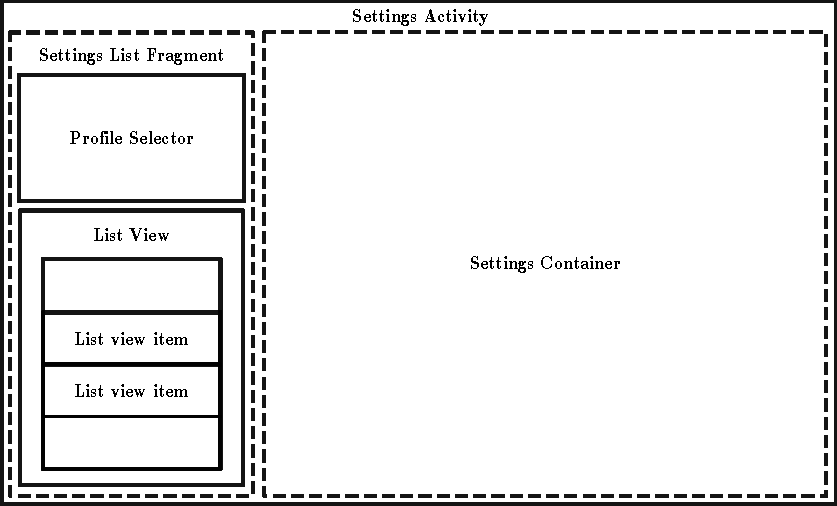
\includegraphics[width=\textwidth, keepaspectratio=true]{SettingsActivity.pdf}
\caption{The architecture showing how the prototype, \cref{fig:settingsprototype}, will be implemented.}
\label{fig:settingsarchitecture}
\end{figure}

Having investigated how to handle settings from other \giraf applications in \cref{sec:sprint3:designsettings}, this sections elaborates on how this is designed following Android terminology taking \cref{fig:settingsprototype} as the underlying basis of the design decisions.

\paragraph{Settings Activity}
Analogous to opening a new window on a desktop computer, a ``screen'' on an Android device consists of an activity.
\Cref{fig:settingsprototype} can be compared directly to \cref{fig:settingsarchitecture}, to expand on the User Interface components that need be included.

To follow Android guidelines we are using fragments\cite{fragments} to implement the functionality this activity requires. They are reusable modules which gives decomposition of the application functionality and UI. By using fragments it is also possible to add multiple fragments to a screen without switching activity.

By following these guidelines for developing an activity it is possible to use the same implementation to show the settings on a smaller screen, this is not a requirement at the moment and therefore this has not been taking into account.\\

As illustrated in \cref{fig:settingsarchitecture} it consists of one fragment, \textbf{Settings List Fragment}, and one container, \textbf{Settings Container Fragment}.\thilemann{this is actually not a fragment, but merely a framelayout with an id of settingscontainer}
The settings list fragment contains the profile selector and a list view, these are described below
\begin{itemize}
\item \textbf{Profile Selector} is what makes it possible to edit settings for multiple users.
The prototype previously mentioned shows a profile selector resembling a drop-down menu.
To follow the multi-project guidelines, a component developed by the group responsible for the GUI library will be implemented instead.
When the selected profile changes, settings activity should be reloaded to reflect the newly selected user's settings.
\item \textbf{ListView} shown the categories of settings which are available for the user.
The fragment attached to each category is presented in the settings container fragment when the category is chosen.
\end{itemize}

\subsection{\launcher Settings}\label{sec:launchersettings}
Following the prototypes (\cref{fig:prototypes}), it is clear that a decision has to be taken for which settings to include for \launcher.
According to the customer meetings (\cref{sec:sprint2:firstmeeting,sec:sprint2:secondmeeting}), the presented design and its functionality received positive feedback.
To build on this idea, the following settings should be included:

\begin{itemize}
\item \textbf{\launcher settings}\\
Since no critical settings are needed for \launcher, it will contain the settings presented in the prototypes, apart from the ability of changing colours for an application (see \cref{sec:sprint2:secondmeeting}).
\item \textbf{Application management}\\
This part of \launcher is more critical as it will be the only way of adding certain applications to \launcher, whether they be an Android or \giraf application.
Thus, this part have the responsible of handling all tasks related to application management.
\end{itemize}


















\subsubsection{Design of "Apps" Settings}\label{sprint3:design:apps}

A requirement from Sprint 2 was a pane in settings, where it can be set up which applications each user has access to.
 \lstinline!SettingsActivity! loads fragments into its container, but because "Apps" should distinguish between \giraf and other Android applications, an additional fragmentcontainer needs to be inserted.
 The idea can be seen visualized in \cref{fig:settingsappfragments}.
 
\begin{figure}[h]
\centering
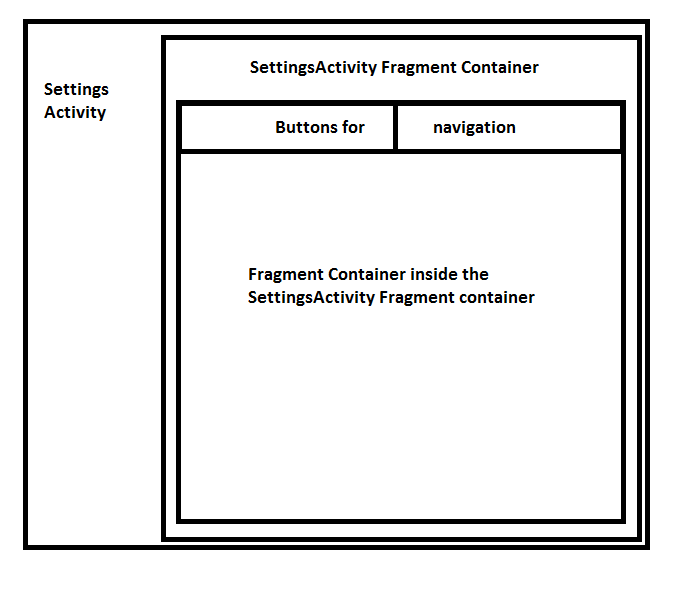
\includegraphics[width=\textwidth, height=3in, keepaspectratio=true] {SettingsActivity.png}
\caption{The organization of \lstinline!SettingsActivity! when inside the "Apps" pane. Since we need to distinguish between \giraf and Android applications, nested fragment containers are used.}
\label{fig:settingsappfragments}
\end{figure}

Because the \giraf and Android pane fragments will contain many of the same variables, these should inherit all shared information from a superclass, consequently reducing redundancy and clarifying how the two fragments are different.

Finally, the navigation buttons inside the \lstinline!SettingsActivity! fragment container should also have a button opening the Google Play Store, so the user can download additional Android applications, if desired. 
Firstly, we researched how to use the inbuilt API for Google Services  to open the Play Store in this way.
However, there were some problems with the API when attempting to implement.
Furthermore, it was discovered that the API is intended to be used for syncronization with Google+, Google Drive and Google Games.
Therefore, we ultimately chose to open the Play Store as a separate activity.\vagner{Please read this and refactor it.}
\subsection{The Appwatcher class}
* | 6b4112c (3 weeks ago) fmikke11@student.aau.dk Added feature to automatically detect and show newly installed applciations.\frederik{Vagner skriver at dette nok skal skrives af Frederik eller Jesper, siden det var dem der lavede den første version af dette.}

\subsection{Guardian only apps no longer requires selecting a child}
| * 84d80e1 (3 weeks ago) jesper.b.kjaer@gmail.com Added constant string of arrays with names of apps that are guardian-only. These apps no longer present a profile selection screen when launched.\\

\section{Developments}
This section described the developments from \cref{sec:sprint3:analysis} in this sprint, primarily focusing on the implementation of settings as described in \cref{sec:sprint3:designsettings}.

\section{Sprint Review}
\subsection{Evaluation}
Implementing the settings was the primary task for the third sprint.
The task consisted of several subtask, which have been completed:

\begin{itemize}
\item It is possible to scale applications up and down and disable the start up animation.
\item It is possible to add and remove both \giraf and Android applications on a 'per user' basis.
\item It is possible to access the Play Store and the native Android settings from settings.
\item It is possible to access the settings of other \giraf applications through \launcher 's settings.
\end{itemize}

This means the task has been solved and the sprint has been a success. 

However, the settings are not as polished as we want them to be.
Therefore, we opted to not present them to the customers at the sprint end, waiting until \launcher is completely done to show our work.\vagner{It could be argued that this is a REALLY bad idea, in terms on official SCRUM practice.}
Sprint end is once again conducted by a member from this group - the details can be found in \cref{collab:sprintend:three}

\subsection{Backlog}

There are some general tasks to be done:

\begin{itemize}
\item The new Profile Selector from \textit{GUI} needs to be implemented.
\item The code base should in general be cleaned up and refactored to ensure structural integrity of the application.
\item The loading animation in \lstinline!MainActivity! statically shows the logo for two seconds and should only be shown for the amount of time it takes to load the needed data.
\end{itemize}

The main task, however, is to refactored and improved the settings:

\begin{itemize}
\item The ListFragment on the left needs to display the chosen pane correctly and proper shadowing should be shown.
\item Loading applications in both \lstinline!GirafFragment! and \lstinline!AndroidFragment! should display a loading animation to the user and load them in a background thread.
\item Installing a new application should update the available ones in \lstinline!GirafFragment! and \lstinline!AndroidFragment!.
\end{itemize}
\chapter{Fourth Sprint}
\vagner{DO NOT WRITE THESE SECTIONS, untill sprint 3 has been written completely.}
\section{Sprint Overview}
The third sprint left a backlog with a number of issues.
These issues are mostly related to either improving the existing code base or the user experience with settings and \launcher in general.
Therefore, this fourth sprint is dedicated to continuing developments from the third sprint and making \launcher a pleasant program to use.

Since the fourth sprint is the last one of this years development of the project, it is different from the other sprints.
First of all, the clients have put a significant emphasis on receiving working applications that do not crash.
While we cannot guarantee that \launcher will not crash during the eights months between the end of this sprint and the beginning of the next, we can improve the code to make \launcher as reliable as possible.\\

After development of the application has been completed, a Usability Test is furthermore carried out to gain insight as to what improvements should be done to \launcher next year.

\section{Analysis and Design}
This sprint was dedicated to polishing the application, both in terms of visual effects and code structure.
The three main elements requiring explanation are:

\begin{itemize}
\item Present time consuming tasks better to the user.
\item Adjusting \launcher to the completed \textit{GIRAF Components}.
\item Incorporation of the remote database.
\end{itemize}

The first element we describe is presenting time consuming tasks in a favourable way to the user.

\section{Developments}
The developments for this sprint does not consider any new developments.
Instead, focus is given to the task of restructuring select classes to improve their readability and make their functionality easier to understand.
Developments from previous sprints are also refactored.

\section{Sprint Review}
\subsection{Evaluation}

As this is the last sprint of the project, \launcher should be completely done and all functionalities should either have been thoroughly tested or disabled.
There is a large emphasis from the clients on receiving  fully working applications that do not crash, as described in \cref{sec:sprint4:sprintoverview}.
We fulfil this requirement by the time the deadline for \launcher is reached.

However, one day before the official Sprint End, the \textit{RemoteDatabase} and \textit{OasisLib} groups declared that synchronization between the two was ready to be implemented.
The details are explained in \cref{collab:sprintend:four}.\\

This is an example of where \launcher is ready and our responsibility towards \launcher is fulfilled.
However, \launcher is dependant on the two database groups and as such, on the multi project level, our responsibility towards having all components of \launcher working is not fulfilled, since synchronizing with the remote database was not implemented when we reached our deadline.

\subsection{Backlog}

The criteria for a successful sprint end was to have fully working applications, that do not crash.
This meant that some functionality is not added in this sprint, as it has not been tested and debugged and we can therefore not be certain that the application will not crash.

As a result, there are some remaining features to be implemented.
Furthermore, there are several ways the existing code can be improved as well.
A thorough description of what can be done by the next group working with \launcher can be found in \cref{sec:eval:futureworks}.
\chapter{Collaboration}\label{chap:collaboration}

\section{Google Analytics}
Google Analytics is a tool for gathering statistics on the use of mobile applications and websites. 
It is developed to help marketers reach their target groups, by analysing how their applications are used.

Most of the possibilites of Google Analytics are not directly relevant to the \giraf project, however it has a feature which could be of great use.
Google Analytics can automatically record uncaught exceptions that occur on the users' devices.
This is a useful feature for multiple reasons. 
The users may not report an application crash to the developers, which prevents the them from addressing the underlying issue. 
Furthermore, Google Analytics continuously monitors problems with the applications, even during the eight months each year, where no students are assigned to the project. 
When a new team of students resume the work, they can immediately start addressing issues that may have shown up during this period.

A member of this group initially came up with the idea of integrating Google Analytics into the \giraf project.
He was made responsible for instructing groups in setting up the tool and make sure that it was implemented correctly.
He also wrote a tutorial, which was distributed to the other groups.

\section{Sprint End Organization}\label{sec:collab:sprintend}
As we are using the Scrum method of development for the entire \giraf project, a sprint review meeting was planned for the end of each iteration. 
\citet[p. 71]{larmanAgile} describes this type of meeting as follows:
\begin{quote}
``At the end of each iteration, there is a review meeting (maximum of four hours)
hosted by the Scrum Master.
The team, Product Owner, and other stakeholders attend.
There is a demo of the product.

Feedback and brainstorming on future directions is encouraged, but no commitments are made during the meeting.
Later at the next Sprint Planning meeting, stakeholders and the team make commitments."
\end{quote}

\subsection{The First Sprint Review Meeting}
At the meeting following the first sprint, the Scrum master of the \giraf project started with a short presentation, and then gave the floor to the groups.
They spent five minutes each demonstrating their progress to the stakeholders. 
After the demonstrations, the stakeholders left, and the groups that would not continue working on the same project (\giraf application) for the next sprint, proceeded to distribute these projects among them, in preparation for the second sprint.

We do not consider this sprint review meeting a success, due to the following reasons:
\begin{itemize}
	\item It was a one-way meeting, where the stakeholders were presented with the progress, but were not encouraged to give any feedback. 
	As a result, the development teams had no gain from the meeting, and were ill prepared for the second sprint. 
	This problem was exacerbated by the lack of the sprint planning meetings required in Scrum to start a new sprint.
	As \citet[p. 70]{larmanAgile} describes, during the sprint planning meetings, goals are re-prioritized and a new sprint backlog is created. 
	\item Several of the demonstrations had technical problems, such as applications crashing in the emulator used for the demonstration.
	This surprised the presenting groups, and thus they were unable to demonstrate their actual progress.
	A related problem was that several groups did not direct their presentation towards the costumers, and therefore focused on technical details, using a very technical vocabulary.
	The demonstration should be better prepared, with more focus on the actual goal of the meeting.
	\item Not all stakeholders were able to attend, as the meeting was planned at a relative late date beforehand.
	As the main goal of the meeting is for the stakeholders to review the progress of the project, this is not optimal.
\end{itemize}

These problems were discussed after the conclusion of the meeting. 
It was suggested that a possible root problem was the \giraf Scrum master being overworked with planning this meeting along with his other responsibilities.
It was decided to, at a later date, discuss the possibility of designating another person as responsible for planning and conducting the sprint review meeting, and possibly the sprint planning meetings as well. Eventually this role was given to a member of this project group.

\subsection{Sprint Review Planning}
\label{collab:sprintend:planning}
To counter the above mentioned points, the new sprint end specialist wrote a directive on how Sprint Review meetings should be performed. Main points in this document include:
\begin{itemize}
	\item The clients should be encouraged to give feedback continually during the meeting, hopefully giving the groups an idea of where their projects are still lacking. Furthermore, the second half of the meeting will consist of a planning phase, where the clients have the opportunity to re-prioritise the goals of the upcoming tasks, or add goals if something important has come up during the meeting. Scrum suggests building the new 	sprint backlog from scratch in cooperation with the clients. We however, see no reason to keep up to nine clients and 60 students in a room for several hours to discuss the sprint backlog, which has to be large enough to keep every student working throughout the upcoming sprint. Instead, one student will compile a preliminary suggestion from the backlog, based on what each group think is the next step for their project. We then give the clients the opportunity to influence this backlog.
	\item The groups are given deadlines for releasing their projects in the versions to be used for the demonstration. Projects that other projects depend upon are to be released to the other groups at least three working days before the sprint review. This gives the other groups a chance to adapt their own projects to the new dependencies. Groups who wish to demonstrate their product to the clients, are to release their final versions at least one working day in advance. This gives the sprint end specialist a chance to collect the applications on a tablet, and let the groups test whether their application works as expected on this tablet. 
	\item To keep the demonstrations on a level that the clients understand, the groups are asked to base their demonstrations on user stories along the lines of ``You are now able to ... by doing ...''. This should prevent the groups from becoming technical in their presentations, and from discussing topics irrelevant to the clients, such as how many hours were spent debugging. 
	\item The dates of the sprint review are advertised to clients well in advance, with a program for the upcoming meeting being sent out at least a week in advance, which should ensure that as many clients as possible are able to attend. 
\end{itemize}

\subsubsection{Install Parties}
At each sprint review meeting, the clients have to bring their Android devices to update the installed \giraf applications to their latest version with the new developments accomplished during the particular sprint.
This is not seen as being an efficient method of distributing updates.
As mentioned in \Cref{sec:collab:localdbtolauncher}, the apps should be avialable through Google Play since this is the correct method to distribute applications to Android devices.
If the applications are distributed through Google Play, the users will automatically get the updates installed on their devices.

\subsection{The Second Sprint Review Meeting}
\label{collab:sprintend:two}
It is difficult to evaluate on the second meeting, as the clients left during a break, due to a misunderstanding. Furthermore, the sprint end specialist was was unable to participate in neither the preparations, nor the meeting itself, so no detailed evaluation of the meeting was conducted. The meeting itself ran into problems, when the clients left the university during an early break, due to a misunderstanding. 

\subsection{The Third Sprint Review Meeting}
\label{collab:sprintend:three}
The third meeting was the first to be executed fully in accordance with the new meeting directive. In the final days before the meeting, the sprint end specialist spent significant amounts of time checking that the various groups finished their demo versions and that the groups tested their applications along with the other applications, in what can be described as an informal integration and system test. 

During the meeting, the sprint end specialist tried to involve the clients in discussions, by asking them open-ended questions. This achieved the affect of making the clients more open to present their thoughts on the various applications. The presentations were much more minded towards the clients, and at a later evaluation of the meeting, it was agreed that the only problem was the presentation skills of some groups, who had some issues with mumbling etc.

The planning phase could be characterised by limited success, as the clients for the most part accepted the suggested backlogs with no comments. A single project had more task suggestions than the group would be able to finish, and the clients were asked directly to opt one out, which they hesitantly did. The problem may have been that they felt awkward telling the groups what to do, and what not to do.

\subsection{The Fourth Sprint Review Meeting}
\label{collab:sprintend:four}
The fourth meeting was somewhat different, as it marked the end of the last sprint, and thus no further developments would be made afterwards. Therefore the time was spent with presenting all the developed applications, while the sprint planning phase was left out. 

The preparations for this meeting became somewhat more chaotic, as it was decided to try making synchronisation between the remote and local databases work. While all deadlines had passed, the day before the meeting, the remote database was declared ready for this step. We decided to go through with it and implement database synchronisation. The expected technical problems showed up, and the overall system became somewhat more unstable, but due to the addition of actual pictograms, we believe it is more useful to the clients than the stable, but empty version we had ready before the integration of database synchronisation. The issues and decisions regarding this, is described in detail in \cref{sec:collab:remotedb}.


\chapter{Evaluation}\label{chap:evaluation}

Overall, we believe \launcher fulfilled the requirements of being a running and working application, when the work was concluded at the end of the last sprint.
We also believe that the collective \giraf suite fulfils this requirement.
There are still issues of reliability, as well as ample opportunity for extending the existing features and adding new ones.
However, especially with the addition of the remote database and its huge collection of pictograms, \giraf is very close to becoming a truly useful tool at the client institutions. 

\section{Multi-project}\label{sec:eval:multiproject}
Reflecting on the multi-project work flow, a number of things could have been improved, and a few things should be retained by later teams. 
The most important ones are described here.

\subsection{Use of Scrum}
\label{sec:eval:multiproject:scrum}
The use of Scrum on the multi-project level did not work out well. 
While Scrum, as described by \citet{scrumGuide}, requires that at least two roles are filled, the Scrum master and the product owner, only a Scrum master was appointed. 

The product owner functions as a representative of the clients' interests, and most importantly manages the product backlog. 
The product owner is therefore vital for keeping development focused, according the needs of the clients.

The Scrum master's task is to facilitate the work of the development team. 
He solves problems the team cannot solve themselves, and handles communication with the rest of the organisation. 
He also coaches the developers in improved organisation and work flow. 
During this iteration of the \giraf project, the Scrum master functioned most of all as a coordinator, as described in \cref{sec:collab:multiproject:roles}. 
It may have given an overall better work flow, if the Scrum master had focused on improving the processes, and enforcing these processes, as to prevent the groups from taking more haphazard approaches to development.

\subsection{Intergroup Communication}
Considering how used the involved groups are to working with single-team projects, the communication between the different groups worked very well. 

While a number of formal communication channels were set up early in the project, most importantly the project management tool Redmine, the groups quickly learned to simply visit each others group rooms when the need to discuss a common issue arose.
This helped preventing a ``them and us'' mentality between groups, and instead helped create a notion of shared responsibility and community. 


\section{Our work process}\label{sec:eval:us}
While it was decided to use Scrum at the multi-project level, the individual groups were free to use other methods.
We chose to adopt Scrum as well.

The morning Scrums provided a great overview of the tasks to be carried out during the day.
Furthermore, the sprint backlog compiled after each sprint, left us with a good overview of tasks to be completed during each sprint.

However, we deviated from Scrum in several ways.

First of all, we did not use a Scrum Master in the group.
Since the group only consisted of four member, it was deemed to be unnecessary.

Second, though we did have sprint backlogs, they were not as detailed as they should be.
This also lead to many tasks appearing during sprints, which were not accounted for in the sprint backlog, and slowed down the group.

Last, the act of estimating the time each task would require was mostly omitted by the group.
While \citet{larmanAgile} points out that this is one of the more difficult parts of Scrum, the group rarely even made an attempt to do so.\\

Despite these deviations, it is the general consensus of the group, that the process, worked well, probably because a group of this small size, generally needs less formal rituals.


The next section discusses further improvements that could be made to the code of \launcher.

\section{Discussion}\label{sec:eval:discussion}
This section discusses the development of \launcher, focusing upon elements that could have been done better.\\

First of all, while a class called \lstinline|Constants| does exist, there are still places in the code where ``magic numbers'' are used.
This fx goes for padding in the \lstinline|AppImageView| class when populating a layout with a list of applications.
A good example is seen in \lstinline|HomeActivity| where instantiating a new \lstinline|TranslateAnimation| to animate a view from on position to another.
The constructor \lstinline|TranslateAnimation(0, to, 0, 0)| does not give any indication to what the 0 mean for each parameter.
Instead, constants defined as a members of the class should have been used: \lstinline|new TranslateAnimation(FROM_X, to, FROM_Y, TO_Y)|, to make the code more readable.

Generally seen, this implies that a good code style should have been established before beginning any developments.
\\

Currently, three utility classes exist, each containing between 100 and 300 lines of code.
The common practice when programming in OO-languages, is to contain methods within classes that use them, and generally not create utility classes.
An example of how this could have been done is to have an \lstinline|AppLayout| class, containing all methods related to populating the layout with applications, which should then be used in \lstinline|HomeActivity| and \lstinline|SettingsActivity| classes.\\


Post development, it is concluded that better decisions according to knowing the general best practices for Android development should have been researched further.
The reason being that the implementation of \lstinline|AppViewCreationUtility| is considered inefficient in the way views are handled.
An optimal implementation would extend the \lstinline|GridView| class.
This would simplify the implementation drastically, since it handles spacing between the views which currently is half of the current implementation.

Reflecting on this, the existing code for handling loading applications into view should have been replaced by another implementation, utilizing an adapter as done with \lstinline|SettingsListAdapter| (\cref{sec:settingslistadapter}).\\

Furthermore, testing should have been done more thoroughly regarding developments from both the last group working with \launcher, but also our new additions.
While functional testing were done during the first sprint (\cref{sec:sprint1:testing}), and informal integration testing before each sprint end (\cref{collab:sprintend:three}), neither system- nor unit tests were explored.
As described in \cref{sec:collab:remotedb}, problems were found according to integrate communication with the Remote Database, which indicates that the informal integration testing should have been more extensively.
Lastly, a code review session with another group would have a positive effect on the code.

\section{A Summary of Future Works}
We found several candidates for improvements of \launcher.
In this section, we only describe the three we deem to have the highest priority.
An exhaustive list of improvements can be found in \cref{appendix:futureworks}.

\paragraph{Copying settings from one user to another} has not been accomplished due to time constraints.
The clients requested the possibility to copy settings from one user to another, this is described in \cref{sec:sprint2:secondmeeting}.
Since this is an actual requirement, we strongly recommend this to be implemented as soon as possible.

\paragraph{Downloading pictograms} while the tablet is being used, is a feature which we find very important.
Currently, when \launcher is started after a system restart, the synchronisation of data with the remote database is executed.
This synchronisation can last up to 30 minutes, during which the user has to wait.
It would be ideal to only download the most essential data, such as profiles and their relations, and thereafter give the user the possibility to login.
\launcher could then continue downloading other data in the background while the tablet is being used.

\paragraph{The loading of applications} into views is suggested to be reimplemented. 
The layout in which applications are being loaded, is currently a linear layout where another linear layout is added acting as a row.
This results in multiple calculations of padding around each application, depending on the chosen icon size.

Instead, the mechanism should be implemented using a grid view.
This makes it possible to add the applications using an adapter and the spacing around the applications would be set automatically.

This increases performance as described in \cref{sec:settingslistadapter}, and would simplify the algorithm used to add the applications to a view significantly.

% Appendices
\appendix
\chapter{Specification Requirements and User Stories}\label{appendix:requirements}
This appendix includes the complete specification requirements and user stories developed during the beginning of the first sprint by one of the multi-project groups.

The original document is included such that four pages are inserted on a single page in the appendix and should be read in a horizontal top-down manner.

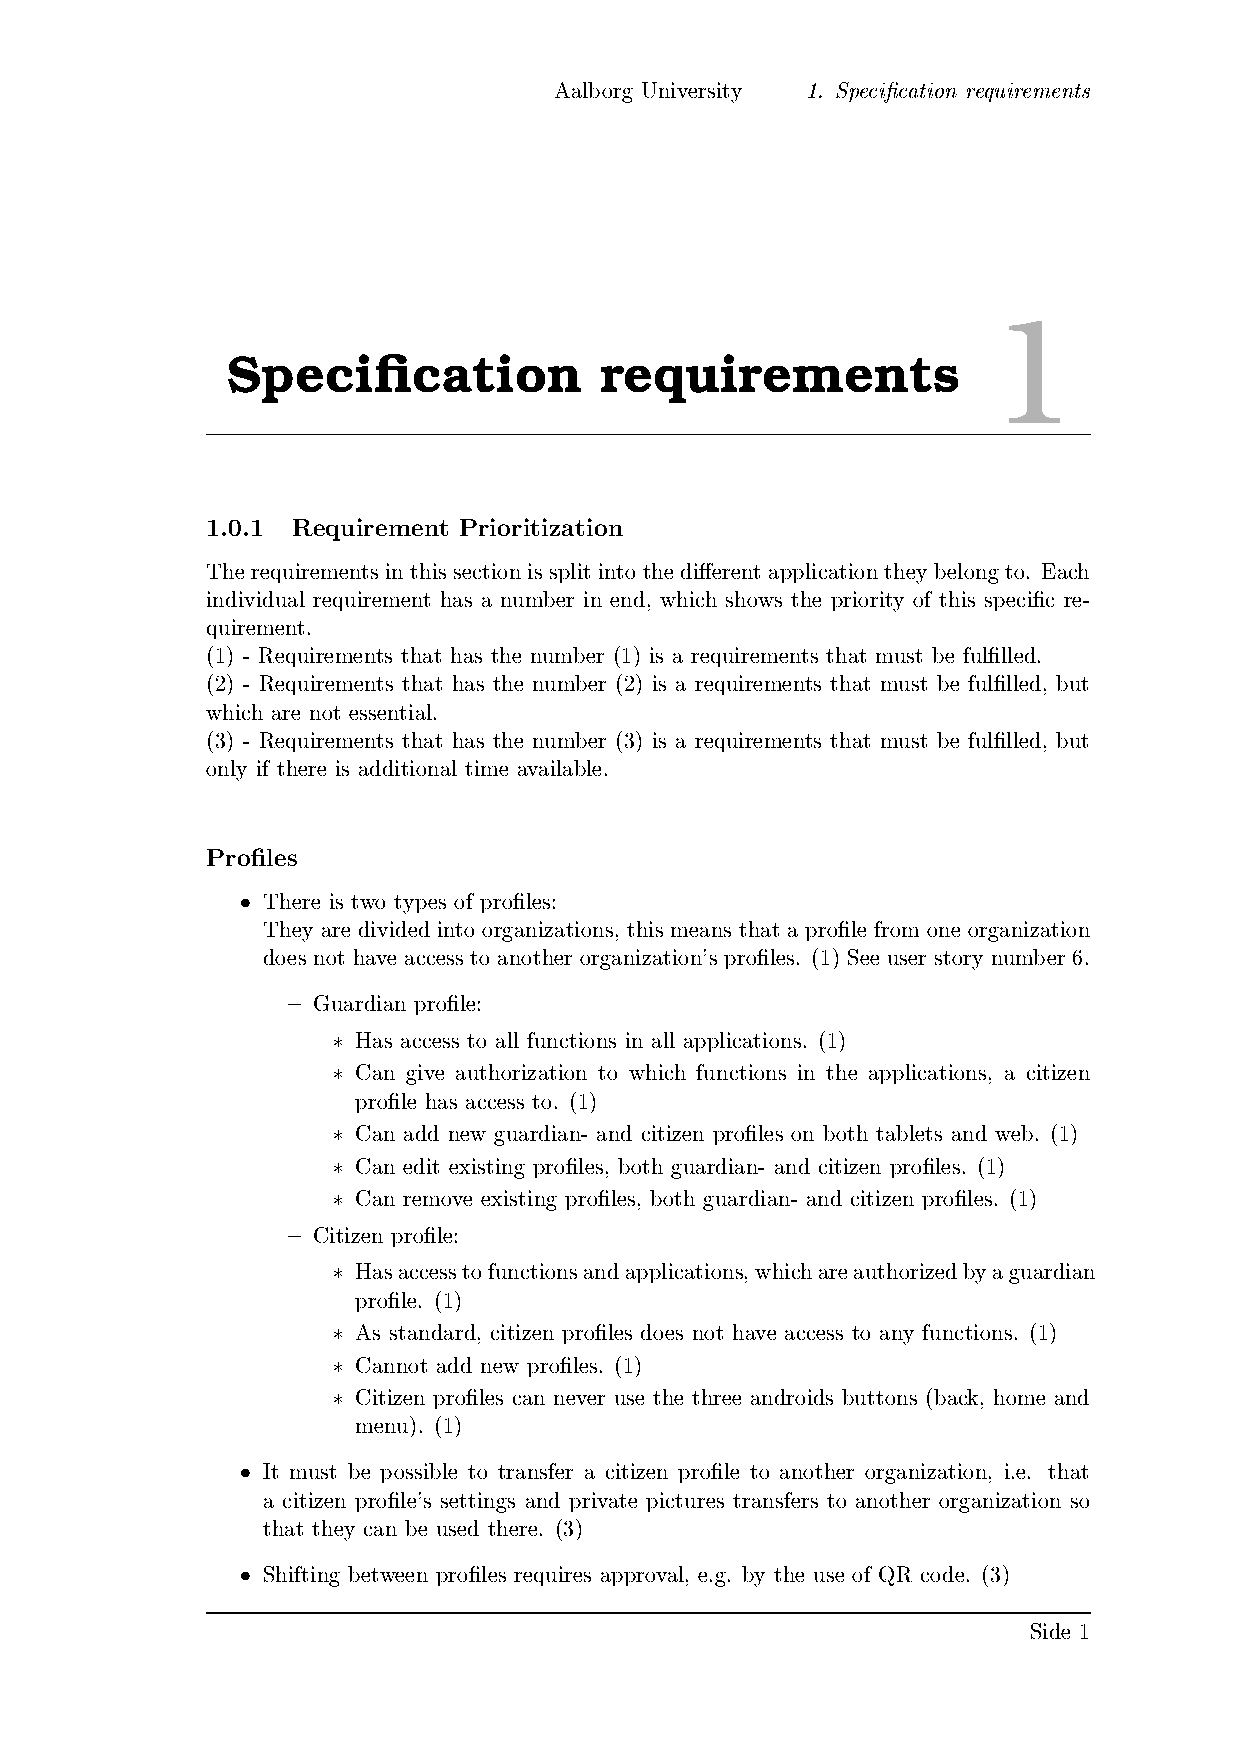
\includepdf[nup=2x2,pages={-}]{documents/Appendix/SpecificationRequirement.pdf}

\chapter{Client Meeting 01-04-2014}\label{appendix:firstmeeting}
\launcher: The point of \launcher is to foreclose the citizens from the rest of the tablets functionality.
It should be as simple as possible.
Pernille thinks it is great that one can change the profile both in the \launcher and inside each individual app.
It is nice that it is the same icon to change profiles everywhere.
There are institutions where everyone have their own tablet and others where the citizens must share.
Pernille thinks that \launcher has the nicest design demonstrated today and that the presentation of how it could work has been very good.
Settings should be individual for each citizen.
Pernille thinks it would be realistic to adjust settings inside each app.
Drazenko just wants it to work.
He believes it provides the best overview to adjust the settings inside each app as well.
However, it is very different how technically adept a citizen is.
``Generelt'' is a bad choice of words under the settings for \giraf.
Pernille wants to know why there is an ability to change colours of apps.
Drazenko thinks it is ok, but not an important feature.
It is probably a good idea to discuss with Birken and bostedet what they meant with their colour requirements.
Generally, people are leaning towards adjusting settings inside each individual app.
Drazenko thinks it is a good idea that external apps can be added to \giraf.
It must be possible to lock which applications can be chosen, so a citizen can not just play everything.
Use a different word than ``Android'', since most are used to iPads.
Another idea is to make an ``Import App'' button like when you insert pictures in a Word document.
Keep it clean and simple!
The drawer becomes irrelevant if the colours are not going to be used.
It is not clear what the purpose of the colours is.
Double check that the requirements from the groups from previous years (If you have any problems with requirements, write me a mail!)
The question is whether or not change of colours is still relevant.
An idea could be to remove the possibility of using other applications for a certain period of time, so a citizen can not switch to a different game while working with another.
Drazenko thinks that \launcher is useful and that it should be simple and grant a good overview.
It should be intuitive how the drawer is opened for change of colour.
Go out and test with the users!
Do not say anything, but observe how they are using it. 
That is really good feedback.
Take pictures so you get some great feedback.

\chapter{Client Meeting 03-04-2014}\label{appendix:secondmeeting}
Check if Android has a feature similar to Apples' ``Restricted Access''.
They like the idea regarding blocking access to other applications while the ``Timer'' is running.
They like the idea regarding profile selection in both \launcher and the individual applications.
They would prefer accessing the settings inside the individual applications.
They like the idea of a collection of settings in \launcher, but they would prefer to have it inside the applications.
They like the feature of creating setting for the guardian and being able copy settings onto the citizen profiles.
They would like both.
They like the idea of being able to bring external applications into \launcher.
They particularly like the idea of disabling and enabling applications for different citizens.
Birken thinks it is okay to see who is logged in.
To change the colours of applications is not a requirement for them.
It is fine with different colours on the applications, but changing colours is not important.

\chapter{Front End Applications}\label{sec:giraf:applications:frontend}
This appendix describes all front end applications in the \giraf suite.

\paragraph{\launcher}
provides an interface for accessing the other tablet applications in a controlled environment, that is easy to use for both guardians and citizens. 
Through \launcher, the guardians should be able to control what applications the citizens should be allowed to use. In the application interface, \launcher is referred to as \giraf.

\paragraph{Sekvens}
allows users to build sentences from pictograms, a central activity in the lives of the citizens \giraf is made to service. Many citizens with autism, especially young children, have difficulty formulating sentences in speech. A central feature of \textit{Sekvens} is also the possibility to save often used sequences of pictograms.

\paragraph{Pictooplæser}
is similar to \textit{Sekvens}, but is focused on building more ad hoc sentences, which the application is then able to read aloud using either an existing recording, or an online text-to-speech tool. 

\paragraph{Kategoriværktøjet}
allows guardians to manage the categories into which the pictograms are organised, including adding and deleting categories and subcategories.

\paragraph{Oasis App}
is an administration tool for manipulating the user information in the database. 

\paragraph{Pictosearch}
is not used as a standalone application, but provides other applications with a common interface for searching through the device's collection of pictograms.

\paragraph{Pictotegner}
allows the user to create their own pictograms with basic graphics tools, such as a free-hand pen tool, a rectangle tool, a circle tool etc. 

\paragraph{Livshistorier}
is also similar to \textit{Sekvens}, but is created specifically for saving pictogram sequences that contain instructions for the citizen's everyday life, e.g. instructions on how to use the bathroom.

\paragraph{Ugeplan}
allows the users to build weekly activity schedules using pictograms. Autistic citizens thrive best in highly strutured environments with regularly scheduled days.

\paragraph{Tidstager}
provides the ability to time an activity, allowing a guardian to let a citizen use an application, e.g. a game, for a set amount of time. When the time runs out, the device locks, forcing the citizen to move on to the next scheduled activity.

\paragraph{Stemmespillet}
is a game, where the citizen controls a car by varying the volume of his or her voice. 

\paragraph{Kategorispillet}
is a game, where the citizen unloads pictograms from a train. The pictograms must be unloaded at different stations, where each station accepts a certain category of pictograms.

\paragraph{Web Ugeplan}
is a web-version of \textit{Ugeplan}, specifically design for large touchscreens. A few costumers had access to TV-size touchscreen, which they specifically wished to use for their week schedules.

\paragraph{Webadmin}
is a web-based administration tool for manipulating the user information in the database.

\chapter{Further code examples}\label{appendix:codeexamples}
This appendix contains code fragments, that are too big to be included as part of the report and that can be omitted..

\section {Debug mode for development}\label{appendix:debugmode}
This section describes the implementation of a debug mode, making developers able to skip certain steps in \launcher, such as the animation screen and the authentication screen.\\

When opening \launcher one is presented \mainactivity, which shows a loading animation, while loading data from the remote database\footnote{Please note, that because the remote database synchronisation was enabled so late in the fourth sprint, debug mode has not been tested.}.
\launcher also requires the users to authenticate themselves, before being given access to the \homeactivity.
While these activities hold meaning in the context of the intended users, a significant amount of debugging time is wasted, as the application is often reinstalled and restarted during development. 

To overcome this problem, we decided to implement a debug mode to simplify and quicken the process of working with \launcher.
The debug mode is controlled from the source code \lstinline|MainActivity| by setting the local fields below (thus, it is not possible to control debug mode at runtime):

\begin{itemize}
\item Enable (true) or disable (false) debug mode entirely, overriding other settings:\\
\lstinline|private final boolean DEBUG_MODE = true;|
\item Skip \lstinline|AuthenticationActivity| activity:\\
\lstinline|private final boolean showAuthentication = false;|
\item Skip the animation on \lstinline|MainActivity| activity:\\
\lstinline|private final boolean showMainAnimation = false;|
\item Login either as a guardian or child when skipping authentication:\\
\lstinline|private final boolean loginAsChild = false;|
\end{itemize}

When the above fields are set, debug mode is enabled globally in \launcher from the \lstinline|onCreate()| method in \lstinline|MainActivity| through the call showed in \cref{lst:debugmode:enable}.

\begin{lstlisting}[caption={Enable debug mode from \lstinline|MainActivity|.},label={lst:debugmode:enable}]  
if(DEBUG_MODE)
  LauncherUtility.enableDebugging(DEBUG_MODE, loginAsChild, this);
\end{lstlisting}

The \lstinline|enableDebugging()| method is seen in \cref{lst:debugmode:enablemethod}.
It needs a reference of the calling activity to show debug information in the active activity.

\begin{lstlisting}[caption={Enable debug mode by calling \lstinline|enableDebugging()|.},label={lst:debugmode:enablemethod}]  
public static void enableDebugging(boolean debugging, boolean loginAsChild, Activity activity) {
  DEBUG_MODE = debugging;
  DEBUG_MODE_AS_CHILD = loginAsChild;

  ShowDebugInformation(activity);
}
\end{lstlisting}

The code in \cref{lst:debugmode:show} is used to set the necessary views, as to inform the developer that debug mode is enabled.

\begin{lstlisting}[caption={Show a debug information on activity if debug is enabled.},label={lst:debugmode:show}]  
public static void ShowDebugInformation(Activity a) {
  if (DEBUG_MODE) {
    LinearLayout debug = (LinearLayout) a.findViewById(R.id.debug_mode);
    TextView textView = (TextView) a.findViewById(R.id.debug_mode_text);
    textView.setText(a.getText(R.string.giraf_debug_mode) + " " + (DEBUG_MODE_AS_CHILD ? a.getText(R.string.giraf_debug_as_child) : a.getText(R.string.giraf_debug_as_guardian)));
    debug.setVisibility(View.VISIBLE);
    try {
      Thread.sleep(200);
    } catch (InterruptedException e) {
      e.printStackTrace();
    }
  }
}
\end{lstlisting}


\section{Launching Google Play}

The code in \cref{lst:launchergoogleplay} describes the \lstinline|OnClickListener| for the \textbf{''Butik''} button in the ''Apps'' pane of settings.
It attempts to open the Play Store app - If it is not installed on the device, it opens Play Store in the browser instead.
\begin{lstlisting}[caption={The OnClickListener for the googlePlayButton, launching the Play Store correctly}, label={lst:launchergoogleplay}]
googlePlayButton.setOnClickListener(new View.OnClickListener() {
	public void onClick(View v) {
		// Try to start the Google Play app
		try {
			Intent intent = new Intent();
			intent.setData(Uri.parse(MARKET_SEARCH_APP_URI + PUBLISHER_NAME));
			intent.setFlags(Intent.FLAG_ACTIVITY_NEW_TASK | Intent.FLAG_ACTIVITY_CLEAR_TOP);
			startActivity(intent);
			// If Google Play is not found, parse the url for Google Play website
		} 
		catch (android.content.ActivityNotFoundException e) {
			startActivity(new Intent(Intent.ACTION_VIEW, Uri.parse(MARKET_SEARCH_WEB_URI + PUBLISHER_NAME)));
		}
	}
}
\end{lstlisting}

\section{Derived class of LoadApplicationTask}

\cref{lst:derivedlat} shows the \lstinline|LoadGirafApplicationTask| - a derived class of \lstinline|LoadApplicationTask|.
The methods of the class calls \lstinline|super.fooBar()| to let the super class carry out most of the work, along with initiating the \lstinline|AppUpdater| in that class and specifying which applications to load.

  \begin{lstlisting}[caption={The LoadGirafApplicationTask, derived from LoadApplicationTask. This is the derived class used by GirafFragment to load applications into view. Please note that all comments and the constructor have been removed to make the listing smaller}, label={lst:derivedlat}]
class LoadGirafApplicationTask extends LoadApplicationTask {
	
	@Override
	protected void onPreExecute() {
		if(appsUpdater != null)
		appsUpdater.cancel();
		
		super.onPreExecute();
	}
	
	@Override
	protected HashMap<String, AppInfo> doInBackground(Application... applications) {
		apps = ApplicationControlUtility.getGirafAppsOnDeviceButLauncherAsApplicationList(context);
		applications = apps.toArray(applications);
		appInfos = super.doInBackground(applications);
		
		return appInfos;
	}
	
	@Override
	protected void onPostExecute(HashMap<String, AppInfo> appInfos) {
		super.onPostExecute(appInfos);
		loadedApps = appInfos;
		startObservingApps();
		haveAppsBeenAdded = true;
	}
}
\end{lstlisting}

\section{Marking GIRAF and Android applications}\label{appendix:markingapps}

\cref{lst:addinggirafapplications} contains the code for marking \giraf applications in the ''Apps'' pane of settings, while \cref{lst:addingandroidapplications} contains the code for marking Android applications in the same pane.

\begin{lstlisting}[caption={The methods used for adding or removing a Giraf application to a user}, label={lst:addinggirafapplications}]
ProfileApplicationController pac = new ProfileApplicationController(context);
ProfileApplication pa = new ProfileApplication(currentUser.getId(), app.getApp().getId());
if(pa == null)
	pac.insertProfileApplication(pa);
else
	pac.removeProfileApplicationByProfileAndApplication(app.getApp(), currentUser);
\end{lstlisting}

\begin{lstlisting}[caption={The methods used for adding or removing an Android application to a user. Please note that the documentation has been removed.}, label={lst:addingandroidapplications}]
String activityName = app.getActivity();

if (selectedApps.contains(activityName))
    selectedApps.remove(activityName);
else
    selectedApps.add(activityName);
\end{lstlisting}

\chapter{Remaining Backlog}\label{appendix:futureworks}
This appendix contains information about the things still remaining to be done in the \launcher project.
As such, it acts as a backlog for the next year bachelor students working on the project.

\section{Proper iconsize}
When scaling the application icons some of them gets pixellated, this indicates that there is still work to be done, when choosing the icons to show. This might be caused by low resolution icons supplied by the developers of the other applications.

\section{Ugeskema Calendarwidget}
The group working on the \textit{GIRAF components} has a widget, showing the current date, in their backlog and it would be an idea to use this widget to open the application \textit{Ugeplan} through this widget. The application should then show the schema for the citizen chosen from the profile selector.

\section{Logging in with citizen and administrator profiles}
Currently, it is possible to login with all types of profiles, but there is no handling of types other than guardian profiles in most of the application.
It might be needed for citizen and administrator login as well.
Citizen profiles should not be able to access certain activities, such as settings in \launcher.
On the contrary, the administrator profiles would need additional access to system administration applications.

\section{Automatically download \giraf applications}
It could be nice to have the \launcher start downloading all \giraf applications as soon as it is started.
This is most likely not possible in Android but it is possible to start Google Play with a search string, meaning that it could be possible to start Google Play with the common part of the Java package name used for the \giraf applications.

\section{Add sound to Launcher}
Currently, none of the actions a user carries out when using \launcher provides audio feedback.
Adding minor sounds for button presses, application launching, setting changes and the like, could be a nice touch to add to \launcher. 

\section{Profile Selection Dialog}
It should be clearly indicated what role, the individual user is assigned, in the list when opening the profile selection dialog.
Currently there are no indication of the role of a user.

\section{Copying settings from one user to another}
For many citizens, the settings may be quite similar.
For this reason, it would be preferable to be able to copy settings from one user to another.

\section{Authentication Activity}
There are still work to do in the authentication activity.

\begin{itemize}
	\item Make it clear that the QR code was successfully scanned.

	An idea is that the camera feed is hidden when the QR code is accepted and who buttons are show, one to scan again and one to login.
	\item Rotation of the instruction animation.

	Currently it is shown as the tablet should be held in portrait mode. For usability matters this should be rotated. %Good luck and have fun with this...!
\end{itemize}

\section{Download pictograms while tablet is being used}
When \launcher is started after a reboot of the device the synchronisation i of data with the remote database is done before being able to login.
If \launcher has never been installed on the device before, this means that it can take up to 30 minutes, before it is ready to login.
It would be an idea to only load the necessary information such as profiles, and then continue downloading the pictograms in the background while the tablet is being used.

\section{GridView used for loading applications}
The container in which applications are being loaded is implemented inconveniently. It should be implemented with a grid view, using a custom adapter. This is better for memory management, and would simplify the algorithm used for showing applications. \frederik{ref til stefans afsnit om adapter i settings}

\label{totalpage}

% Bibliography
\label{biblo}
\bibliography{sources}

%Count the last page	
\label{lastpage}
\end{document}